\documentclass[11pt]{article}
\usepackage[a4paper, hmargin={2.8cm, 2.8cm}, vmargin={2.5cm, 2.5cm}]{geometry}
\usepackage{eso-pic} % \AddToShipoutPicture
\usepackage{graphicx} % \includegraphics
\usepackage{amsmath}
\usepackage{tabto}
\usepackage{amsthm}
\usepackage{hyperref}
\usepackage{xurl}
\usepackage{enumerate}
\usepackage{txfonts}
\usepackage{graphicx}
\usepackage{float}
\usepackage{listings}
\usepackage[space]{grffile}
\usepackage{tabularx} % \For resizing tables
\usepackage{color, colortbl}
\usepackage{xcolor}
\usepackage{multicol}
\usepackage{caption}
\usepackage{subcaption}
\usepackage{minted}
\usepackage{titlesec}

\setcounter{secnumdepth}{4}

\newtheorem{theorem}{Theorem}[section]
\theoremstyle{definition}
\newtheorem{definition}{Definition}[section]
\titleformat{\paragraph}
{\normalfont\normalsize\bfseries}{\theparagraph}{1em}{}
\titlespacing*{\paragraph}
{0pt}{3.25ex plus 1ex minus .2ex}{1.5ex plus .2ex}


\usepackage[style=authoryear]{biblatex}

\DeclareFieldFormat{postnote}{p. #1}
\addbibresource{bib.bib}
\setlength\bibitemsep{1.5\itemsep}

\lstset { %
    language=C++,
    backgroundcolor=\color{black!5}, % set backgroundcolor
    basicstyle=\footnotesize,% basic font setting
}
\hypersetup{breaklinks=true}

%% Change `ku-farve` to `nat-farve` to use SCIENCE's old colors or
%% `natbio-farve` to use SCIENCE's new colors and logo.
\def \ColourPDF {include/ku-farve}

%% Change `ku-en` to `nat-en` to use the `Faculty of Science` header
\def \TitlePDF   {include/nat-en}  % University of Copenhagen

\title{
  \vspace{3cm}
  \Huge{Differential Privacy} \\
  \Large{Implementation and examination of four differential privacy models}
}

\author{
  \Large{Friis, Jonas}
  \\ \texttt{jof1007@gmail.com} \\
\texttt{xdr476@alumni.ku.dk}
}

\date{
    \today
}

\begin{document}

\AddToShipoutPicture*{\put(0,0){\includegraphics*[viewport=0 0 700 600]{\ColourPDF}}}
\AddToShipoutPicture*{\put(0,602){\includegraphics*[viewport=0 600 700 1600]{\ColourPDF}}}

\AddToShipoutPicture*{\put(0,0){\includegraphics*{\TitlePDF}}}

\clearpage\maketitle
\thispagestyle{empty}

\newpage

%% Write your dissertation here.
\section{Abstract}
In this thesis, we present and discuss central and local differential privacy for range counting and the amount of noise added to the output; We do this by implementing different central and local differential private data structures. We implement a flat solution in both central and local DP. We furthermore examine two variations of hierarchical histograms. The data structures are implemented in Python. We then analyze and benchmark the data structures against each other by measuring the error over different range queries. 


\newpage
\tableofcontents
\newpage
%%%%%%%%%%%%%%%%%%%%%%%%%%%%% Introduction %%%%%%%%%%%%%%%%%%%%%%%%%%%%%
\section{Introduction}
Current companies collect and use their users/customers' data to improve and develop their services. It makes sense for the company to want their users/customers' data. In that way, the company can develop products that the users/customers want to utilize instead of guessing (speculating) what they may want. However, the data that the companies collect about their users could potentially be personal information that the users do not want to share. Therefore the users will demand privacy guarantees. \\

\noindent There have been several naive attempts to preserve the privacy of the users.  One simple naive (One such?) approach would be to simply strip the data from personally identifying information, such as names, addresses, social security numbers, etc. This approach usually fails; the leftover data can be used in connection to other data/information from different datasets to identify people uniquely. This linkage attack was first done back in 2000 by Latanya Sweeney, who identified the former Governor of Massachusetts  William Weld's health records using his date of birth, gender, and zip code (\cite{Sweeney}). Another example of this occurred in 2007 when Netflix released a dataset of 100,480,507 ratings that 480,189 users gave to 17,770 movies, where they removed personally identifying information and changed some ratings. Attackers were able to recover 99\% of personal data using auxiliary data from IMBD (\cite{netflix}). \\

\noindent This tells us that all data can potentially be personally identifying information. We can not make the assumption that an adversary sees the dataset in isolation. Neither do we know what kind of auxiliary data the adversary has access to or how an adversary plans to use the data. Therefore it does not make sense to focus on making some specific data set private;  instead, we should focus on the algorithms/techniques that we use to analyze the data; when doing so, we will get more meaningful guarantees about privacy.  These analysis algorithms/techniques are called differential private.\\

This thesis examines the fundamentals of differential privacy and implements different differential privacy data structures, and measure the noise added to the data. \colorbox{blue}{this text}
% What this points to is that, rather than focusing on making a particular set of data private (e.g., through de-identification by removing personally identifying information), the scientific community has discovered that making an analysis technique (or algorithm) private provides more meaningful guarantees. 

% Seeing a data set in isolation makes it hard, if not impossible, to decide whether the data are successfully de-identified. As we observed already, this depends on what an attacker trying to re-identify individuals knows, and what additional information may be available from other sources. Without knowing who may try to do the re-identification, and what information they possess, or which individuals or what new information they are interested in, we cannot decide if a data set is safe for publication. If we know, however, the method (e.g., the algorithm) through which the data was analyzed to produce some by-product of it, such as a table of counts or a machine learning model, then we can actually make guarantees that hold against any possible attacker, with any kind of side information. This insight was developed initially in work by Dwork, McSherry, Nissim, and Smith [9], who introduced a seminal framework for private data analysis known as differential privacy. Differential privacy has seen an increasing number of recent adoptions, both in industry (by Google, Apple, Facebook, among others) and by official statistics agencies, most notably the U.S. Census Bureau starting with the 2020 Decennial Census.

%     rather than focusing on making a particular set of data private (e.g., through de-identification by removing personally identifying information), the scientific community has discovered that making an analysis technique (or algorithm) private provides more meaningful guarantees.

% As we mentioned, differential privacy defines privacy with respect to an algorithm used to analyze data, rather than with respect to the data themselves. 

% Informally, the definition can be described using a thought experiment. Imagine that we execute the algorithm on a data set, and we also execute it on the data set with the data of one individual modified. To be differentially private, the algorithm must behave almost identically in these two scenarios, and this must happen for all data sets and all modifications to the data of any one individual. For example, a differentially private algorithm must have the property that if it produces a particular machine learning model from a data set that includes your data, then it is almost as likely to produce the same model if your data were removed or changed completely. This means that an adversary observing or using the model output by this algorithm is unable to tell whether your data (or any other person’s data) were used to train the model at all. Then, whatever information an attacker may learn about you from observing the algorithm’s output could have also been learned even if your data were never seen by the algorithm. 

% Differentially private algorithms have the property that they reveal statistical information about the data, such as, for example, correlations between genetic factors and medical conditions, but do not reveal information about particular individuals, such as whether they have some medical condition. This is because statistical information does not depend crucially on any one person’s data, while private personal information does. We should note that the actual technical definition is quantitative, and the level of privacy protection is tunable, allowing us to trade privacy off for the machine learning model’s accuracy, or to query answers produced by the algorithm.

% Let us illustrate this with a short example of how differential privacy can be achieved. Suppose we just want to release two counts, such as our previous examples “How many computer science professors at the University of Toronto smoke?” and “How many computer science professors at the University of Toronto who were not born in Bulgaria smoke?” Then we can add some random noise to each count, for example by flipping some number of coins and adding the number of tails we get to the first count, and doing the same with new coins for the second count. Now, even if an attacker subtracts the two noisy counts from each other, the result they get will be dominated by the random noise, and they cannot tell if this blog post’s authors smoke. The more coins we flip, the better the privacy protection. At the same time, we can achieve good privacy protection with many fewer coin flips than the number of computer science professors at the University of Toronto, giving us reasonably accurate answers to the two counting questions.
% Conclusion 

% Given what the scientific community has learned about the risks of re-identification attacks, and about defining privacy protection rigorously, we advocate that de-identification be interpreted in terms of how data is analyzed. Combined with proper access control measures to ensure that the data themselves are not directly accessible, analyzing data with algorithms that provide rigorous guarantees of privacy allows us to envision a future where respectful, yet nevertheless useful, applications of data analysis are possible.


\section{Problem definition}
When releasing datasets to the world that contain sensitive personal attributes, the aggregator who releases the data should make sure that no information from an individual subject of the dataset could be gained from an adversary. To archive this, the aggregator can use different mathematical techniques that yield differential privacy.
This project focuses on range counting, which is defined as processing an object S, in order to determine how much of the object intersects with a query called the range. Examples could be how many individuals of a dataset are male or how many are between the ages 20 and 25. The general technique to archive differential privacy when releasing answer to range counting is by the addition of random noise to it. When doing this, we get private range counting.

In this project, the aim is to examine some of the techniques to archive differential privacy and how these techniques can be used in combination. Furthermore, we want to implement these techniques in a localized differential privacy model and a centralized differential privacy model. Use the implementations to make experiments on how much noise they add to the answer and how effective they are on a real dataset when doing private range counting.

%%%%%%%%%%%%%%%%%%%%%%%%%%%%%%% Notation %%%%%%%%%%%%%%%%%%%%%%%%%%%%%%%
\section{Notation}
A short list of notations used throughout the thesis:
\begin{itemize}
\item DP = differential privacy
\item $F$ = Frequency oracle
\item $V_{F}$ = Variance of frequency oracle
\item $\hat{\theta}[j]$ = Estimator of point $j$ when using a frequency oracle
\item $\theta[j]$ = True value of point $j$ 
\item $Lap(b)$ to denote a random variable $X\sim Lap(b)$.

\end{itemize}

\section{Differential Privacy}
The purpose of this section is to first introduce concepts about differential private algorithms and then give a informal definition. Next, we lead this into a mathematical definition of differential private algorithms, and explain a central and local model of computation. 
\subsection{Sensitivity of a DP algorithm}
Before we talk about the sensitivity a DP algorithms, we will first introduce how we think about databases.
We will think of databases $z$ as being collections of records from a domain $\mathcal{Z}$. The way we want to use databases is that we would want to think about their histograms, which are $z\in N^{|\mathcal{Z}|} $, each entry $z_i$ represents the number of elements in the database $z$ of type $i\in \mathcal{Z}$. We will now introduce a measure of the distance between two databases z and y. We will be using the the 1 norm/distance. The 1 norm of a database x is 
\[\lVert z \rVert_1 = \sum_{i=1}^{|\mathcal{Z}|} | z |_1\]
Then the 1 norm of two databases x and y is $\ell_1 = \lVert x-y \rVert_1$
\[\lVert x-y \rVert_1 = \sum_{i=1}^{|\mathcal{Z}|} | x |_1-| y |_1\]
The 1 norm is a measure of how many records differ between x and y. The sensitivity of a function $f$ is defined by the 1 norm. The 1 norm captures how much a single record, a individual persons data can change the function $f$ in the worst case. The magnitude of the 1 norm is the 'amount of randomness' we need to introduce in the function $f$, in order to preserve the privacy the participation of a single individual. A formal definition would be; the sensitivity of a function gives an upper bound on how much we must perturb its output to preserve privacy (\cite[17]{algo_fun}).

% We will think of databases $x$ as being collections of records from a universe $\mathcal{X}$. It will often be convenient to represent databases by their histograms $x:\in N^{|\mathcal{X}|} $, in which each entry $x_i$ represents the number of elements in the database $x$ of type i∈X(we abuse notation slightly, let-ting the symbol N denote the set of all non-negative integers, including zero). In this representation, a natural measure of the distance between two databases x and y will be their`1distance:Definition 2.3(Distance Between Databases). The`1norm of a database x is denoted |x| 1and is defined to be:‖x‖1=|X|∑i=1|xi| .The`1distance between two databases x and y is|x-y|1 Note that |x| 1 is a measure of the size of a database x(i.e., the number of records it contains), and  $||x-y||$1 is a measure of how many records differ between x and y. Databases may also be represented by multisets of rows(elements of X) or even ordered lists of rows, which is a special case of a set, where the row number becomes part of the name of the element. In this case distance between databases is typically measured by the Hammingdistance, i.e., the number of rows on which they differ. However, unless otherwise noted, we will use the histogram representation described above. (Note, however, that even when the histogram notation is more mathematically convenient, in actual implementations, the multiset representation will often be much moreconcise).

% The `sensitivity of a function $f$ captures the magnitude by which a single individual’s data can change the function f in the worst case, and therefore, intuitively, the uncertainty in the response that we must introduce in order to hide the participation of a single individual. Indeed, we will formalize this intuition: the sensitivity of a function gives an upper bound on how much we must perturb its output to preserve privacy. One noise distribution naturally lends itself to differential privacy.
% For a DP algorithm:

% the sensitivity of f is:

% on datasets d1, d2 differing on at most one element.

% The above definition is quite mathematical, but it’s not as bad as it looks. Roughly speaking, the sensitivity of a function is the largest possible difference that one row can have on the result of that function, for any dataset. For instance, in our toy dataset, counting the number of rows has a sensitivity of 1, because adding or removing a single row from any dataset will change the count by at most 1.

\subsection{An Informal Definition}
One way to try defining privacy from the context of data analysis is to require that the adversary does not know more about any of the individuals in the data set after the analysis is performed than the adversary knew before she/he got the analysis results. This goal is formalized by requiring that the adversary's prior knowledge and posterior knowledge about an individual should not be 'too different', or that access to the database should not change the adversary's views about any individual 'too much'.
The appeal of this notion to defining privacy is that if nothing is learned about an individual, then the individual cannot be harmed by the analysis. However, that is impossible; if this requirement should be achieved, the database does not contain any information, and then why should the adversary query this database for information? Thus, this notion of privacy is unachievable.


\subsection{A Formal Definition}
We first explain where the privacy comes from. The privacy comes from a process, where there is introduced some randomness, which is often done via random sampling, adding noise and linear transformations. With this stated we move on to a technical definition of differential privacy.
\subsubsection{Definition Of Epsilon differential privacy}
To define what it means for an algorithm to be differential private, we must first define a randomized algorithm.\\ A randomized algorithm $M$ with domain $A$ and discrete range $B$ is associated with a mapping $M:A\rightarrow\Delta(B)$. On input $a\in A$, the algorithm $M$ outputs $M(a) =b$ with probability $(M(a))_b$ for each $b\in B$.
A randomized algorithm $M$ gives $(\epsilon,0)$ -differential privacy if for all databases $D$ and $D'$ differing on at most one row, and any $S \subseteq Range(M)$,
\[
\operatorname{Pr}[\mathcal{M}(D) \in \mathcal{S}] \leq \exp (\epsilon) \operatorname{Pr}[\mathcal{D'}(x) \in \mathcal{S}]
\]
We can see there are two quantities we must consider in DP algorithms: \\ $\epsilon$: The metric of privacy loss at a differentially change in data (adding, removing one entry). The smaller the value is, the better privacy protection. \\ Accuracy: How much the output of DP algorithms differ from the true output.
We can think of the parameter $\epsilon$ as determining the overall privacy protection. This roughly translates to the increase of the risk of individuals' privacy has of being compromised. A smaller value for $\epsilon$ implies better protection. This also translates the other way around; a larger value for $\epsilon$ gives worse protection. If we let $\epsilon = 0$ we would have perfect privacy; not a single individual in the analysis have risked their privacy at all. However, if we have $\epsilon = 0$ in the real world, the output would only consist of noise and, therefore, the analysis would be useless.

\subsection{What differential privacy does promise}


Differential privacy gives a promise to the data holder from the aggregator, that any participant will not be inflicted with any harm stemming from the fact that they released their data to aggregator's private database $x$. Thus, a participant could still face harm. However differential privacy gives the guarantee that the probability of harm was not significantly increased by their choice to release their data. %This gives an individual no reason not to give their data to the aggregator's private database, because 
% What differential privacy promises An Economic View.Differential privacy promises to protect individ-uals from anyadditional harm that they might face due to their data being in the private database x that they would not have faced had their data not been part of x. Although individuals may indeed face harm once the results M(x)of a differentially private mechanism M have been released, differential privacy promises that the probability of harm was not significantly increased by their choice to participate. This is a very utilitarian definition of privacy, because when an individual is deciding whether or not to include her data in a database that will be used in a differentially private manner, it is exactly this difference that she is considering: the probability of harm given that she participates,as compared to the probability of harm given that she does not participate. She has no control over the remaining contents of the database.Given the promise of differential privacy, she is assured that she should 

% be almost indifferent between participating and not, from the point of view of future harm. Given any incentive — from altruism to monetary reward — differential privacy may convince her to allow her data to be used. This intuition can be formalized in a utility-theoretic sense,which we here briefly sketch.Consider an individuali who has arbitrary preferences over the set of all possible future events, which we denote by A. These preferences are expressed by a utility function ui:A →R≥0, and we say that individuali experiences utility ui(a)in the event that a∈ A comes to pass. Suppose thatx∈N|X|is a data-set containing individualis private data, and thatMis anε-differentially private algorithm. Let y be a data-set that is identical to x except that it does not include the data of individuali(in particular,‖x−y‖1= 1), and le t f: Range(M)→∆(A)be the (arbitrary) function that determines the distribution over future event s A, conditioned on the output of mechanism M. By the guarantee of differential privacy, together with the resilience to arbitrary post-processing guaranteed by Proposition 2.1,we have:Ea∼f(M(x))[ui(a)] =∑a∈Aui(a)·Prf(M(x))[a]≤∑a∈Aui(a)·exp(ε)Prf(M(y))[a]= exp(ε)Ea∼f(M(y))[ui(a)]Similarly,Ea∼f(M(x))[ui(a)]≥exp(−ε)Ea∼f(M(y))[ui(a)].Hence, by promising a guarantee ofε-differential privacy, a data analyst can promise an individual that his expected future utility will not be harmed by more than an exp(ε)≈(1+ε)factor. Note that this promise holds independently of the individualis utility function ui, and holds simultaneously for multiple individuals who may have completely different utility functions.

%1However, as the group gets larger, the privacy guarantee deteriorates, and this is what we want: clearly, if we replace an entire surveyed population, say, of cancer patients, with a completely different group of respondents, say, healthy teenagers, we should get different answers to queries about the fraction of respondents who regularly run three miles each day. Although something similar holds for(ε,δ)-differential privacy, the approximation termδtakes a big hit, and we only obtain (kε,ke(k−1)εδ)-differential privacy for groups of size k.

\subsection{What differential privacy does not promise}
While differential privacy does deliver a strong guarantee about preserving privacy, it can not promise there can not be done harm. It can not create privacy out of thin air. Differential privacy does not guarantee that secrets disclosed in the survey will remain secret. It ensures that an individual's participation in a survey will not in itself be disclosed, nor will participation lead to the disclosure of any results that one has answered within the survey. However, if there are enough participants, the survey will disclose statistical information about the population who took the survey. The statistical information the survey obtains can then be used to draw conclusions.

The purpose of any survey is to discover statistical information about a population so we can draw conclusions about the population; if any of these conclusions hold for a given individual, it does not mean that we have violated differential privacy; Forall intends and purposes the individual may not even have participated in the survey. Differential privacy sets a guarantee that these results would be obtained with a very similar probability of whether or not the given individual participated in the survey.

\subsection{Composition theorems}
We will now examine what happens if we use two differentially private algorithms in combination. We will see that the output of this will also be differentially private, this comes of the consequence that $\epsilon$ will degrade and leading to a increase of the accuracy. Consider that we repeatedly compute the same thing/statistic, with the Laplace mechanism or a frequency oracle from the sections \ref{lap} and \ref{freq} respectively. The mean of all the answers given by the DP algorithms will eventually converge to the true value of the thing/statistic, and so we cannot avoid the fact that the strength of our privacy guarantee will degrade with repeated use. To proof this we will first show that two independent use of an $\epsilon_1$-differentially private algorithm and an $\epsilon_2$-differentially private algorithm, when taken together, is $(\epsilon_1+\epsilon_2)$-differentially private. The proof follows here: \\
We let $M_1:N^{|X|} \rightarrow R_1$ be an $\epsilon_1$-differentially private algorithm, and $M_2:N^{|X|} \rightarrow R_2$ be an $\epsilon_2$-differentially private algorithm. Then their combination, defined to be $M_{1,2}:N^{|X|}\rightarrow R_1\times R_2$ by the mapping: $M_{1,2}(x) = (M_1(x),M_2(x))$ is  $\epsilon_1+\epsilon_2$-differentially private algorithm. We fix the databases $x,y \in N^{|X|}$, we fix two points in the domain $(r_1,r_2)\in R_1\times R_2$
\begin{align*}
    \frac{\operatorname{Pr}\left[\mathcal{M}_{1,2}(x)=\left(r_{1}, r_{2}\right)\right]}{\operatorname{Pr}\left[\mathcal{M}_{1,2}(y)=\left(r_{1}, r_{2}\right)\right]} &=\frac{\operatorname{Pr}\left[\mathcal{M}_{1}(x)=r_{1}\right] \operatorname{Pr}\left[\mathcal{M}_{2}(x)=r_{2}\right]}{\operatorname{Pr}\left[\mathcal{M}_{1}(y)=r_{1}\right] \operatorname{Pr}\left[\mathcal{M}_{2}(y)=r_{2}\right]} \\
&=\left(\frac{\operatorname{Pr}\left[\mathcal{M}_{1}(x)=r_{1}\right]}{\operatorname{Pr}\left[\mathcal{M}_{1}(y)=r_{1}\right]}\right)\left(\frac{\operatorname{Pr}\left[\mathcal{M}_{2}(x)=r_{1}\right]}{\operatorname{Pr}\left[\mathcal{M}_{2}(y)=r_{1}\right]}\right) \\
& \leq \exp \left(\varepsilon_{1}\right) \exp \left(\varepsilon_{2}\right) \\
&=\exp \left(\epsilon_{1}+\epsilon_{2}\right)
\end{align*} \\
We use this fact to show that $i$ independent $M_i$ mechanisms that are $e_i$-differentially private algorithms, used in combination, will result in a mechanism $M_k$ that are  $\sum_i^K\epsilon_i$ $e_i$-differentially private.\\ Let $\mathcal{M}_{i}: \mathbb{N}^{|\mathcal{X}|} \rightarrow \mathcal{R}_{i}$ be an $\left(\varepsilon_{i}, 0\right)$ -differentially private algorithm for $i \in[k]$. Then if $\mathcal{M}_{[k]}: \mathbb{N}^{|\mathcal{X}|} \rightarrow \prod_{i=1}^{k} \mathcal{R}_{i}$ is defined to be $\mathcal{M}_{[k]}(x)=\left(\mathcal{M}_{1}(x), \ldots, \mathcal{M}_{k}(x)\right)$, then $\mathcal{M}_{[k]}$ is $\left(\sum_{i=1}^{k} \varepsilon_{i}, 0\right)$ -differentially private.

\subsection{Central Differential Privacy}
In central differential privacy, there is a trusted aggregator who holds the entire dataset of all individual users; these can be thought of as rows. Each user then reports their row to this aggregator. The aggregator then wants to keep every individuals row private \colorbox{blue}{this text}. The aggregator then uses a DP algorithm on the data which has been sent. Here we only add randomness in one place, which makes this model very accurate. The disadvantage is that the aggregator knows all actual data, which means the user really has to trust the aggregator enough to share its data with it. To obtain the trust needed for this can however be difficult. The aggregator could be an untrustworthy company or government. In the central model, the aggregator collects all the data in one place. This increases the risk of catastrophic failure e.g. if the aggregator gets compromised and leaks all the data.
This model of computation can be seen on Figure \ref{fig:model_cen_dp}.
\begin{figure}[H]
    \centering
    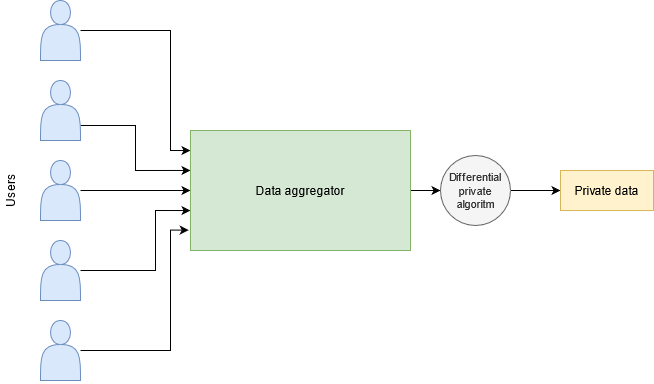
\includegraphics[width = .8\textwidth]{figures/DP_cen.png}
    \caption{Model of central differential privacy}
    \label{fig:model_cen_dp}
\end{figure}

\subsection{Local Differential Privacy}\label{teo_local}
Initial work on differential privacy assumed the presence of a trusted aggregator, who curates all the private information of individuals, and releases information through a DP algorithm; this was explained in the previous section.  In practice, individuals may be reluctant to share private information with a data aggregator. This could be because the user does not trust the aggregator or worries that the aggregator could be sold to someone they do not trust in the future. It could also be that it is hard to gain trust due to the nature of the information, e.g., a survey about illegal activities. The local variant of differential privacy is where the user only knows their data, a local view of the dataset. The users then independently release information about their data through a DP algorithm. This model of computation can be seen on Figure \ref{fig:model_local_dp}. They can even release the whole dataset while still be being differential private. Since each user adds noise to their data, this will increase the overall noise by a considerable margin over the central model. This generally means we need a lot more users to report their data to learn something about the population. \\

When working with local differential privacy, there arises another problem/consideration; the communication cost needs to be considered. The communication cost is the amount of data the aggregator, and a user have to exchange. We would want the communication cost to be as low as possible. This could come at the expense of some computation on both the user and aggregator ends.
\begin{figure}[H]
    \centering
    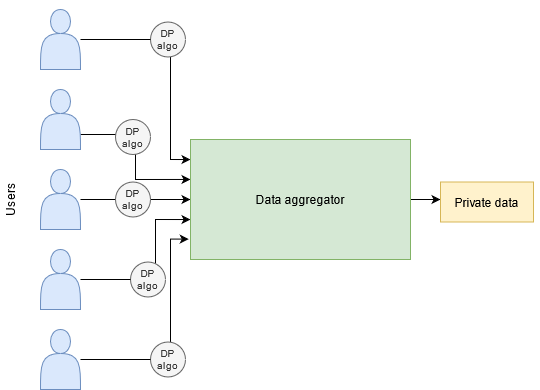
\includegraphics[width = .8\textwidth]{figures/DP_local.png}
    \caption{Model of local differential privacy}
    \label{fig:model_local_dp}
\end{figure}


\section{Point and range queries}
What we would want to in this project is to focus on differential private range counting. Range counting, is defined as processing an object $S$, in order to determine how much of the object intersects with a query called the range. We will start by looking at point queries instead of range queries, as point queries are just range queries with range 1. With point queries, we try to estimate the frequency of of a element single element $z$ in a domain $\mathcal{Z}$. 
% We next formally define the range queries that we would like to support. As in Section 3.2, we assume N non-colluding individuals each with a private item zi∈[D]. For any a<b,a∈[D],b∈[D], a range query R[a,b]≥0is to compute R[a,b]=1NNÕi=1Ia≤zi≤bwhereIpis a binary variable that takes the value 1 if the predicate p is true and 0 otherwise. Definition 4.1.(Range Query Release Problem) Given a set of N users, the goal is to collect information guaranteeing ε-LDP to allowapproximation of any closed interval of lengthr∈[1,D]. Let b R be an estimation of interval R of length r computed using a mechanism F. Then the quality of F is measured by the squared error(b R−R)2.
Then if we want to a range query, we can just sum up the $z$ in our range. A range query has the sensitivity of 1, an individual data can only change the count by one. 

\section{Data Structures For Central Differential Privacy}
In the central model, we know the frequency of all the elements in our domain. We now wish to make this frequency differential private. To make the frequency of all the elements differential private, we will introduce some random noise. The noise will be drawn from the Laplace distribution. We will then add this noise to the true frequency $z$; this will be named the Laplace mechanism.

\begin{definition}[Laplace mechanism]\label{lap}
Given any function $f:\mathbb{N}^{|Z|}\rightarrow \mathbb{R}^k$, the Laplace mechanism is defined as: \[f(x) + (Y_1,...,Y_k)\]
where $Y_i$ are i.i.d. random variables drawn from $\operatorname{Lap}(\frac{\Delta f}{\epsilon})$ and $\Delta f$ is the sensitivity of the function, in the case for counting, the sensitivity is $\Delta f=1$.
\end{definition}
The proof for Laplace mechanism preserves $(\epsilon, \ 0)$ differential privacy is as follows.
Let $x\in\mathbb{N}^{|X|}$ and$y\in\mathbb{N}^{|X|}$ be such that  $\lVert x-y\rVert_1\leq 1$, and let f(·) be some function $x\in\mathbb{N}^{|X|}\rightarrow \mathbb{R}^{k}$. Let $p_x$ denote the probability density function of $ML(x,f,\epsilon)$, and let $p_y$ denote the probability density function of $ML(y,f,\epsilon)$. We then compare the two at some arbitrary point $z\in\mathbb{R}^{K}$
\begin{align*}
\frac{p_{x}(z)}{p_{y}(z)} &=\prod_{i=1}^{k}\left(\frac{\exp \left(-\frac{\varepsilon\left|f(x)_{i}-z_{i}\right|}{\Delta f}\right)}{\exp \left(-\frac{\varepsilon\left|f(y)_{i}-z_{i}\right|}{\Delta f}\right)}\right) \\
&=\prod_{i=1}^{k} \exp \left(\frac{\varepsilon\left(\left|f(y)_{i}-z_{i}\right|-\left|f(x)_{i}-z_{i}\right|\right)}{\Delta f}\right) \\
\intertext{Using the triangle inequality gives us }
& \leq \prod_{i=1}^{k} \exp \left(\frac{\varepsilon\left|f(x)_{i}-f(y)_{i}\right|}{\Delta f}\right) \\
&=\exp \left(\frac{\varepsilon \cdot\|f(x)-f(y)\|_{1}}{\Delta f}\right) \\
\intertext{We have that $\Delta f = 1$ and $\lVert x-y\rVert_1\leq 1$  }
& \leq \exp (\varepsilon) 
\end{align*}
Which is fulfills the definition of $\epsilon$-differentially private algorithm.



\subsection{Central Flat Solution}\label{teo_cen_flat}
An obvious way to support range queries would be to use the Laplace mechanism $\operatorname{Lap}(\epsilon)$ at each of the true frequencies and then simply sum up the estimated frequency in the range. The variance at each frequency is, therefore, $V_\mu=\frac{2}{\epsilon^2}$. We let $|r|$ denote the number of frequencies we want to sum up. Then we get that the expected error is $\mathrm{Var}(E_m (r))=r\cdot V_\mu$, which means the variance is linear with respect to the length of the query. The average length of the interval $N$ is $\frac{\sum_{i=1}^{N} i(N-i+1)}{N(N+1) / 2}=\frac{(N+2)}{3}$ which means the average error would be $\frac{(N+2)}{3}\cdot V_\mu$.

\subsection{Continuous Observation}
A different way to support range queries would be to support continuous observation of a count; in our case, each day would be the domain $\mathcal{Z}$ and store the counts at each element in the domain $\mathcal{Z}$. Then to support range queries, we would simply need to subtract the count at the last element of the range query and subtract the first count in the range. \\ \\
In the book \cite{algo_fun} at page 243, they have a data structure to support exactly this. It works that we need the domain $|\mathcal{Z}|$ to be a power of 2. Then every interval are the natural ones corresponding to the labels on a complete binary tree with $|\mathcal{Z}|$ leaves, the leaves are labeled, starting from the left and going right, with the intervals $[0,0],[1,1],...,[T-1, T-1]$ and each parent is labeled with the union of the interval of its children. To compute the noisy count for each leave $[t_1,t_2]$  \colorbox{blue}{noisy count}; that is, the value corresponding to the label $[t_1,t_2]$, we have a tree of the same dimensions where each leave is i.i.d $\operatorname{Lap}(\frac{1 + \log_2 |\mathcal{Z}|}{\epsilon})$, we then compute the path down to our node $[t_1,t_2]$ and add each Laplace variable on the way, this is then the noisy count for leave $[t_1,t_2]$. To learn the count of an element in the domain, we sum the nodes in the B-adic decomposition of the range. To answer a range query, we do need two elements in the domain and subtract them from each other. The pseudocode for the algorithm can be seen in Figure 12.1 on page 243 in the book \cite{algo_fun}. \\ \\
Now we show why this ensures $(\epsilon,0)$-differential privacy; we know each element in the domain appears at most $1 + \log_2 |\mathcal{Z}|$ intervals as the height of the tree is $log_2 |\mathcal{Z}|$. So every element in the domain can only affect the output $1 + \log_2 |\mathcal{Z}|$ times. Then if we add noise to each leaf distributed according to $\operatorname{Lap}(\frac{1 + \log_2 |\mathcal{Z}|}{\epsilon})$ it ensures $(\epsilon,0)$-differential privacy. This argument is easily extended for other than a binary tree. This data structure is almost identical to the local hierarchical histogram we will describe later on. \\

\colorbox{blue}{this text} It is important reuse the same Laplace variables for the noisy counts and not sample some new ones. First I implemented a data structure where I sampled new Laplace variables for every count. This is however not DP, because we can let the size domain get really big to increase the height of the tree. Then the law of large numbers tells us the Laplace variables would cancel out as they mean $0$.

\section{Data Structures For Local Differential Privacy}
In contrast to the central case, we do not know the true count at each point.
Each user $i$ holds a private element $z_i$ from the domain $\mathcal{Z}$. This domain can be describes as a unknown discrete distribution $\theta$, where $\theta_z$ is the probability that a randomly sampled input element is equal to $z\in\mathcal{Z}$. We want have a local DP protocol so the aggregator can estimate $\theta$ as $\hat{\theta}$ as accurately as possible.
\subsection{Frequency Oracle}\label{freq}
Solutions for this problem are referred to as providing a frequency oracle. There have been several suggestions of frequency oracles described in recent years. In each case, the users perturb their input on their own data (locally), often via linear transformation or random sampling, and send the result to the aggregator. The noisy reports each user reports are aggregated together and corrected by the expected noise to reconstruct the frequency for each item in $\mathcal{Z}$. The estimators for these mechanisms are unbiased and have the same variance with the same bias $V_f$ for all items in the input domain (\cite[3]{local}). \\

\noindent Three different versions of frequency oracle is described on page 3 of \cite{local} . Where the focus of this thesis will be of the one they call modified Optimal Local Hashing (OLH). In the paper they use hashing to reduce the communication cost between the individuals and the aggregator. In contrast, when I will be using the frequency oracle, I will both be the individuals and the aggregator so there are no communication cost. There is also a flaw in the paper as it seems they ran out of symbols to use, where they use $g$ for two things, both the hashing range and the variable to minimise the variance of the frequency oracle in a way that contradict each other. The frequency oracle works as such, with  probability $\frac{e^{\epsilon}}{e^{\epsilon}+g-1}$ the individual answer truthfully or else reports a value sampled u.a.r from the domain. The aggregator then collect all the individuals reports and  computes a frequency vector for all items in the original domain, based on what was reported from all $N$ individuals. All $N$ such histograms are added together to give $T\in\mathbb{R}^D$. The aggregator then uses the unbiased estimator $\hat{\theta}(i)= \frac{T[i] - (1-p) \cdot \frac{N}{g} }{p}$ to get the frequency for all elements in the original domain, the variance should is  $V_f= O\left(\frac{e^{\epsilon}}{N\left(e^{\epsilon}-1\right)^{2}}\right)$ (\cite[3]{local}). 

\subsection{Local Flat Solution}
The flat solution for local DP, is almost the same as with central DP, instead of adding the noise of Laplace, the permutation comes from the frequency oracle. 
We can see that for an interval $[a,b]$, we let the range be $R_{[a,b]}=\sum_{i=a}^b f_i$, where is our estimated frequency $f_i$ of $i\in \mathcal{Z}$. This frequency is estimated by our frequency oracle. Therefore a simple approach is to sum up estimated frequencies for every item in the range. The error behaves exactly the same way as in the central flat solution.


\subsection{Local Hierarchical Histogram}
Before looking at hierarchical histogram, we introduce the notion of B-adic intervals and a property of B-adic decompositions. An B-adic intervals if it is on the form  $k B^{j} \ldots(k+1) B^{j}-1$ for $j\in [log_BD]$ and $B\in\mathbb{N}^+$. Any subrange of in a B-adic intervals of length $r$  can be decomposed into max  $(B-1)\left(2 \log _{B} r+1\right)$ sub intervals. \\ \\
If we look at the range query problem as representing answering collections of histograms, each element in the domain is a bin. In the local flat solution we have bin for each element. This leads to an error that is linear in the length of the range. We can ask oneself what if we keep some bins for the subranges of the domain instead of having a bin for all of the domain. A way to do this is impose a hierarchy on the domain items in such away that the frequency of each item contributes to multiple bins. With this structure we should be able to answer, queries by adding counts from a smaller number of bins. \\ \\
In the hierarchical histograms, we arrange the intervals into a tree with branching factor b, where the unit-length intervals are the leaves, and each node in the tree corresponds to an interval that is the union of the intervals of its children. An illustration of the nodes subranges in a hierarchical histograms with an degree of two can be seen on Figure \ref{fig:disjoint}.
\begin{figure}[H]
    \centering
    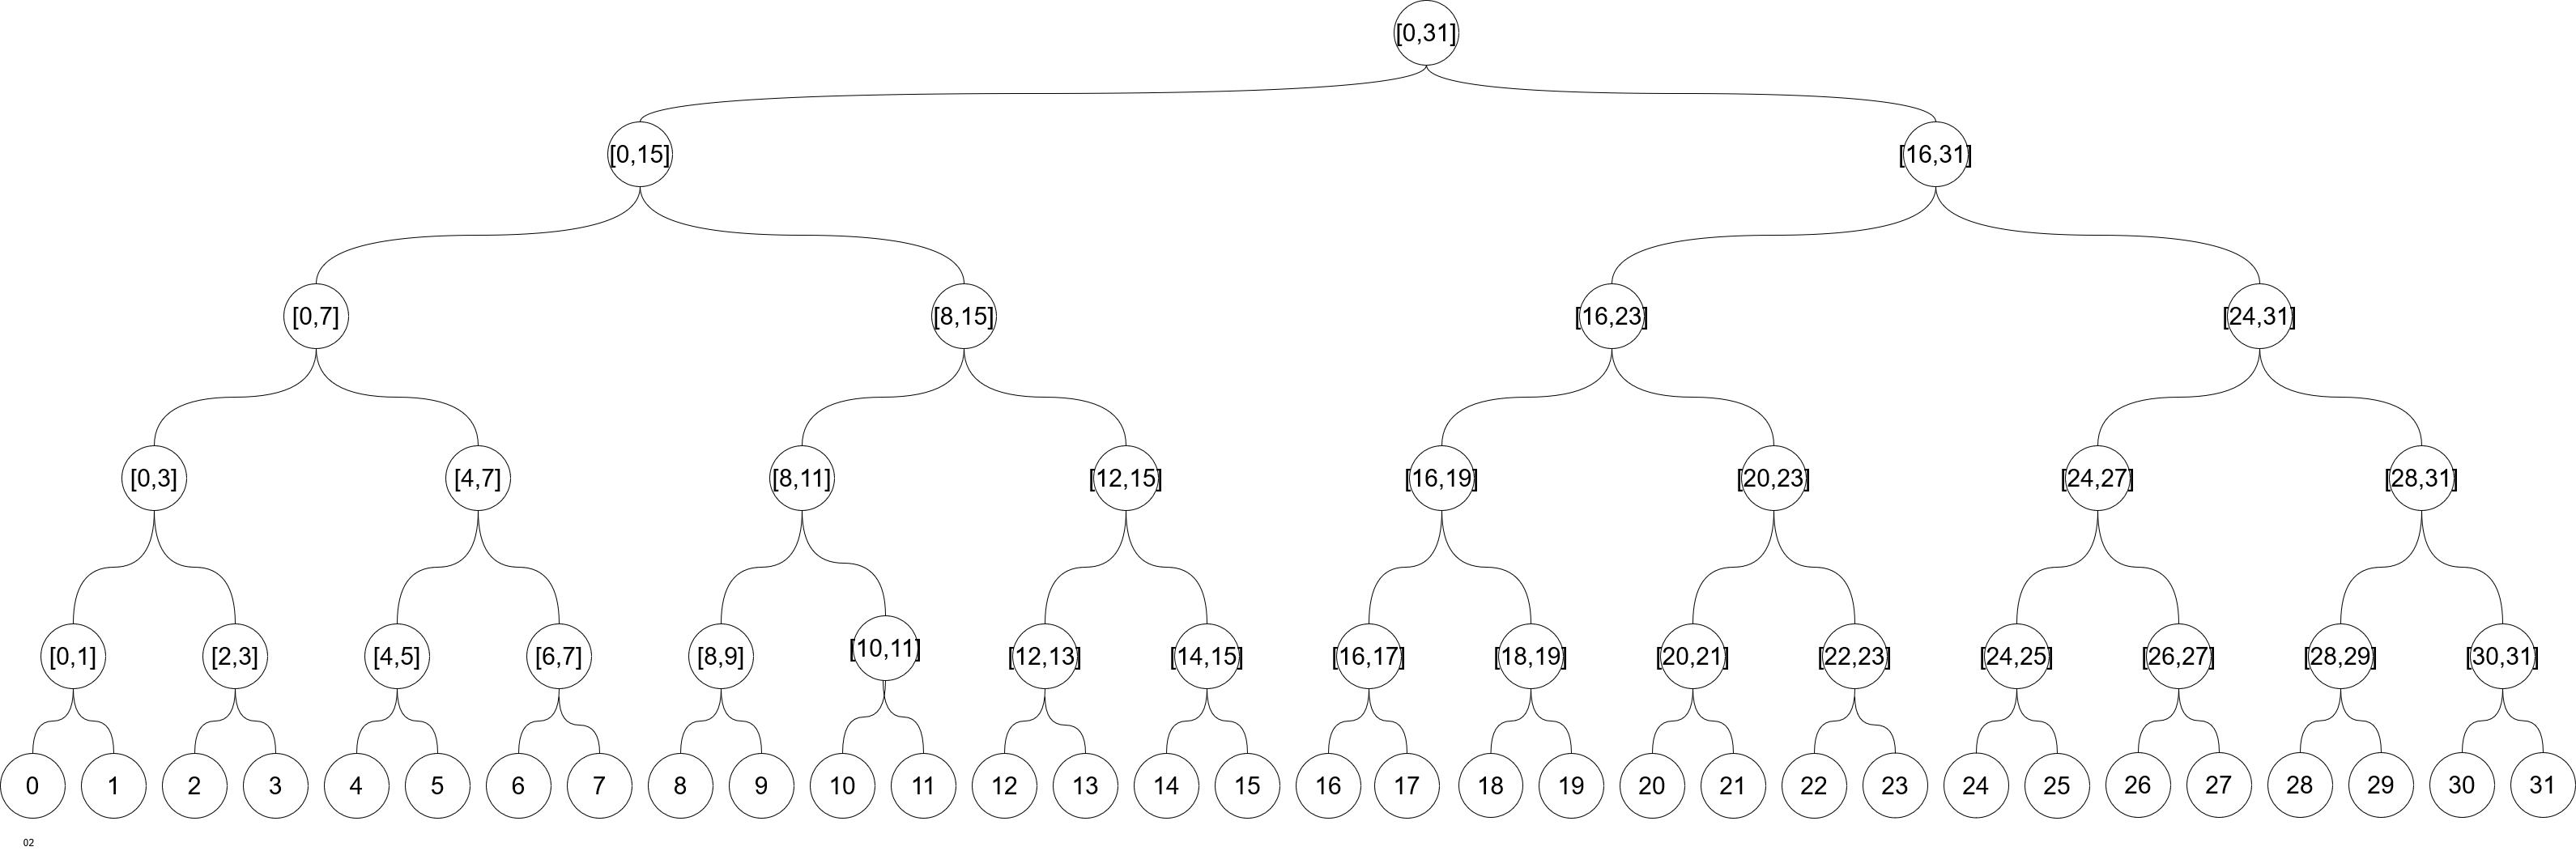
\includegraphics[width=.8\linewidth]{figures/disjoint_tree.png}
    \caption{Hierarchical histograms representation}
    \label{fig:disjoint}
\end{figure}
Each user $i$ has an item $z_i$ from the domain, $z_i$ will match with a leaf in the bottom of the tree. The user $i$ arranges their input $z_i\in \mathcal{Z}$ as a full tree of height with degree $B$. $z_i$ will have a unique path from leaves to the root with a weight of 1 attached to each node on the path, and zero elsewhere, see Figure \ref{fig:sub1} for the local view with  $z_i=2$ and $b=2$.  We can therefore see each level in the tree as a vector with 1 in one place and zero everywhere else. Hence, we can use our frequency oracle from section \ref{freq}, all the levels.  \\ \\

\noindent I will now present the steps that the users has to do. \\
User $i$ samples a random level with probability $p_l$, then 
perturbs this vector using the frequency oracle, reports the perturbed information to the aggregator along with what level it was, see Figure \ref{fig:sub2} for an example of a perturbation of level 3 with $z_i=2$. \\ \\
\noindent I will now present the steps that the aggregator has to do. \\
The aggregator builds the same empty tree and adds what each individual contributes to the corresponding nodes. The aggregator answer a range query by using the frequency oracle estimator on the nodes from the B-adic decomposition of the range and times it with height of the tree to compensate for the random sampling of levels. Something to note here is that we loose a little piece of information by doing this. We only add data to one node in the path, but we still know the path up in the tree as it is identified by all parents of the nodes. We could not do something similar with the children of this node as we do not known which of the children leaf we should contribute to. 

\begin{figure}[H]
\centering
\begin{subfigure}{.5\textwidth}
  \centering
  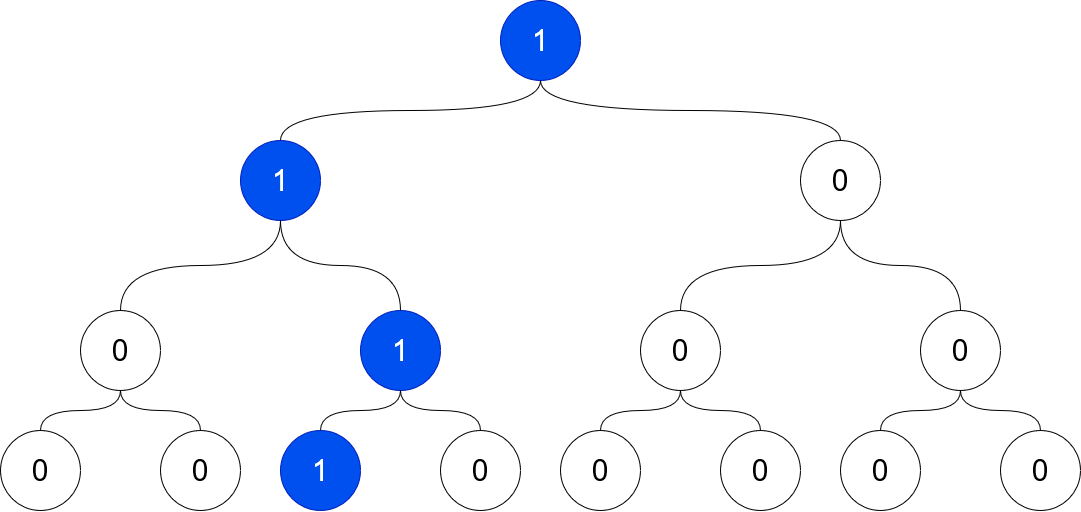
\includegraphics[width=.8\linewidth]{figures/binary_tree_path_1.png}
  \caption{Local view with $z_i=2$}
  \label{fig:sub1}
\end{subfigure}%
\begin{subfigure}{.5\textwidth}
  \centering
  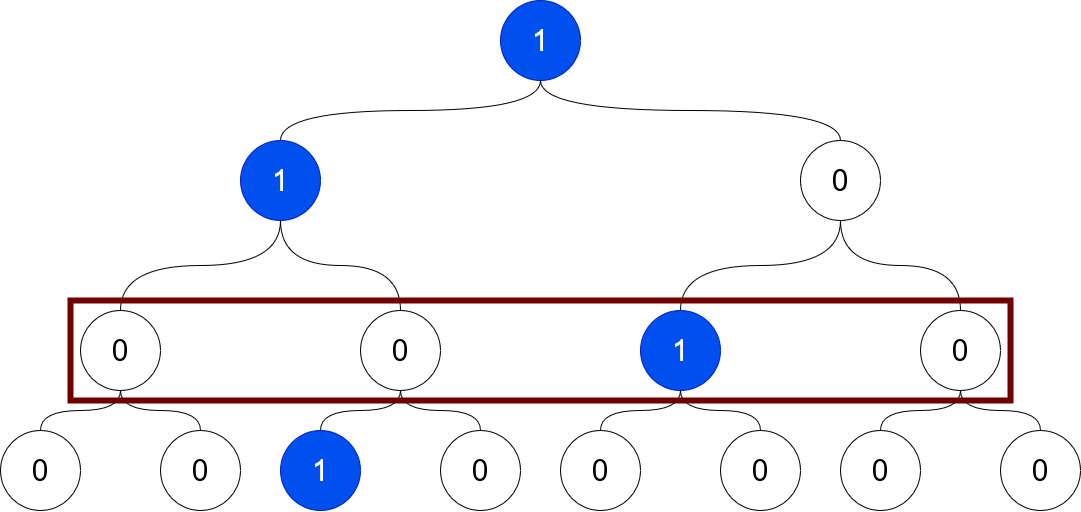
\includegraphics[width=.8\linewidth]{figures/binary_tree_path_1_sample.png}
  \caption{Local view with $z_i=2$ and perpetuated level 3}
  \label{fig:sub2}
\end{subfigure}
\caption{Local view with $z_i=2$ and perpetuation}
\label{fig:binary_tree}
\end{figure}
\subsubsection{Error for Local Hierarchical Histograms}
We denote hierarchical histograms with degree B as $HH_B$. First we show that overall variance can be expressed by the variance of the frequency oracle, $V_f$.  We remember that the variance of the frequency oracle is $V_f= O\left(\frac{e^{\epsilon}}{N\left(e^{\epsilon}-1\right)^{2}}\right)$ where $N$ is the amount of people contributing to the frequency oracle. Here we observe that the variance does not depend on the domain, which in our case is size of the levels, the variance depends only the amount of people who contributed to the frequency oracle. We can then introduce $V_F\leq\psi_F(\epsilon)/N$ where $\psi_F(\epsilon)$ is a constant for method the frequency oracle that depends on $\epsilon$. This gives us the ability to fix the variance for all nodes in any to be in the same level to be $V_l$. $V_l$ the variance of a given level is determined by how many users randomly sample that level $N_l$. We remember that the range query of length $r$ is decomposed into at $2(B-1)$ nodes at each level, we can at maximum use $\alpha=\lceil log_B r\rceil+1$ levels. This gives the bound of total variance to be \[\sum_{l=1}^{\alpha}(2 B-1) V_{l}=\sum_{l=1}^{\alpha}(2 B-1) V_{F} / p_{l}=(2 B-1) V_{F} \sum_{l=1}^{\alpha} \frac{1}{p_{l}}\]
It can further be proven that to minimise variance we need to set $p_{l}=\frac{1}{h}$, which means the users sample their level uniformly at random (\cite[5]{local}). \\ \\

\noindent We can further optimise the error by adjusting our degree $B$ of the $HH_B$. This comes from the fact that a larger degree will Ireduce the height of the tree. This will increases accuracy of estimation per node since larger fraction of the users is allocated to each level. But doing this, it also means that we require more nodes at each level to evaluate a query which we have shown increases the total error. 

\section{Implementation}
The code can be found in the appendix and also on the GitHub page: \url{https://github.com/jfriisKU/Bachelors-Thesis}, the zip file and in appendis here \ref{app:imp}. The code was implemented in python 3.6
The following python libraries have been used in the implementations: 
\begin{multicols}{2}
\begin{itemize}
    \item Numpy
    \item Pandas
    \item datetime
    \item scipy
    \item matplotlib
    \item os
    \item Re
    \item sys
    \item psycopg2
\end{itemize}
\end{multicols}

The numpy library allows us to quickly and nicely manipulate arrays. \\ The domain of the dataset dates, therefore we need a library to handle that, pythons standard library datetime was chosen to handle this. \\ The psycopg2 library allows us to interact with a PSQL database. This was needed as we loaded our dataset into PSQL database to access of the data in different python files. \\ 
The library scipy allows us get an implementation of the Laplace distribution where we could control the scale of the distribution. This was need in both of the implementation of the central models, which relies on the Laplace distribution. \\
The library matplotlib made plotting and showing the results much quick and easy. \\
Os, Re and sys was mainly used for saving and loading the results from the experiments on the data structures for further analysis.

\subsection{Generally for all data structures}
In all the implemented data structures, I have saved the true count of every element. This was done to make the experiments and the later analysis much easier, as we can ask the data structure what the true answer was and saved it with the estimation. 

\subsection{Central flat solution}
The implementation for the Central flat solution, takes three arguments $\epsilon$, the domain and the counts of each element in the domain. 
When running the implementation, the data structure adds $\operatorname{Lap}(\epsilon)$ to every count and saves this count in a new array. This new array is then used to answer the range queries, by summing up every element given in the range.

\subsection{Local flat solution}
The implementation for the local flat solution, takes three arguments $\epsilon$, the domain and the counts of each element in the domain. We represent the domain as a 1d array, where each element in the array corresponds to element in the domain. When running the implementation, the data structure, estimates the frequency in the domain, we use the frequency oracle on every count in each element in of the domain. The frequency oracle reports element of the domain, we then add one our estimation of the frequency in the domain. The array of noisy counts the frequency oracle produced is then, used to answer the range queries, we use the unbiased estimator on every element given in the range, and sum them up when doing a range query. 

\subsection{Answering Queries In Hierarchical Histograms}\label{decom}
As noted in the previous section about continuous observation and local hierarchical histograms. The two data structures do not differ that much in concept. They both answer range queries by making use B-adic decomposition. In both the Continuous Observation and local Hierarchical Histograms, I did not make the B-adic decomposition, but i opted for another way for finding the leaves in the B-adic decomposition. \\ \\
One can instead look at it as a binary search down the tree after the nodes just before and after the range. When we search for a node just before our range then every time we go to the left child, we need to count the node at our right. When we search for the node just after our range, then every time we go to the right child, we need to count the node at our left. After doing this search we have found all the nodes we need in our B-adic decomposition.\\ \\
An example of this is given here, say we are interested in the range $[2,22]$ and we have $B=2$ and $D=32$, this range can be decomposed into $|2,3| \cup|4,7| \cup|8,15| \cup|16,19| \cup|20,21| \cup|22,22|$. This search in the tree is illustrated in Figure \ref{fig:disjoint_se_1}, where the green line is the search for node right before our query and the purple line is the search for our node right after our range. The nodes in the red circles are the ones we want to count. 
\begin{figure}[H]
    \centering
    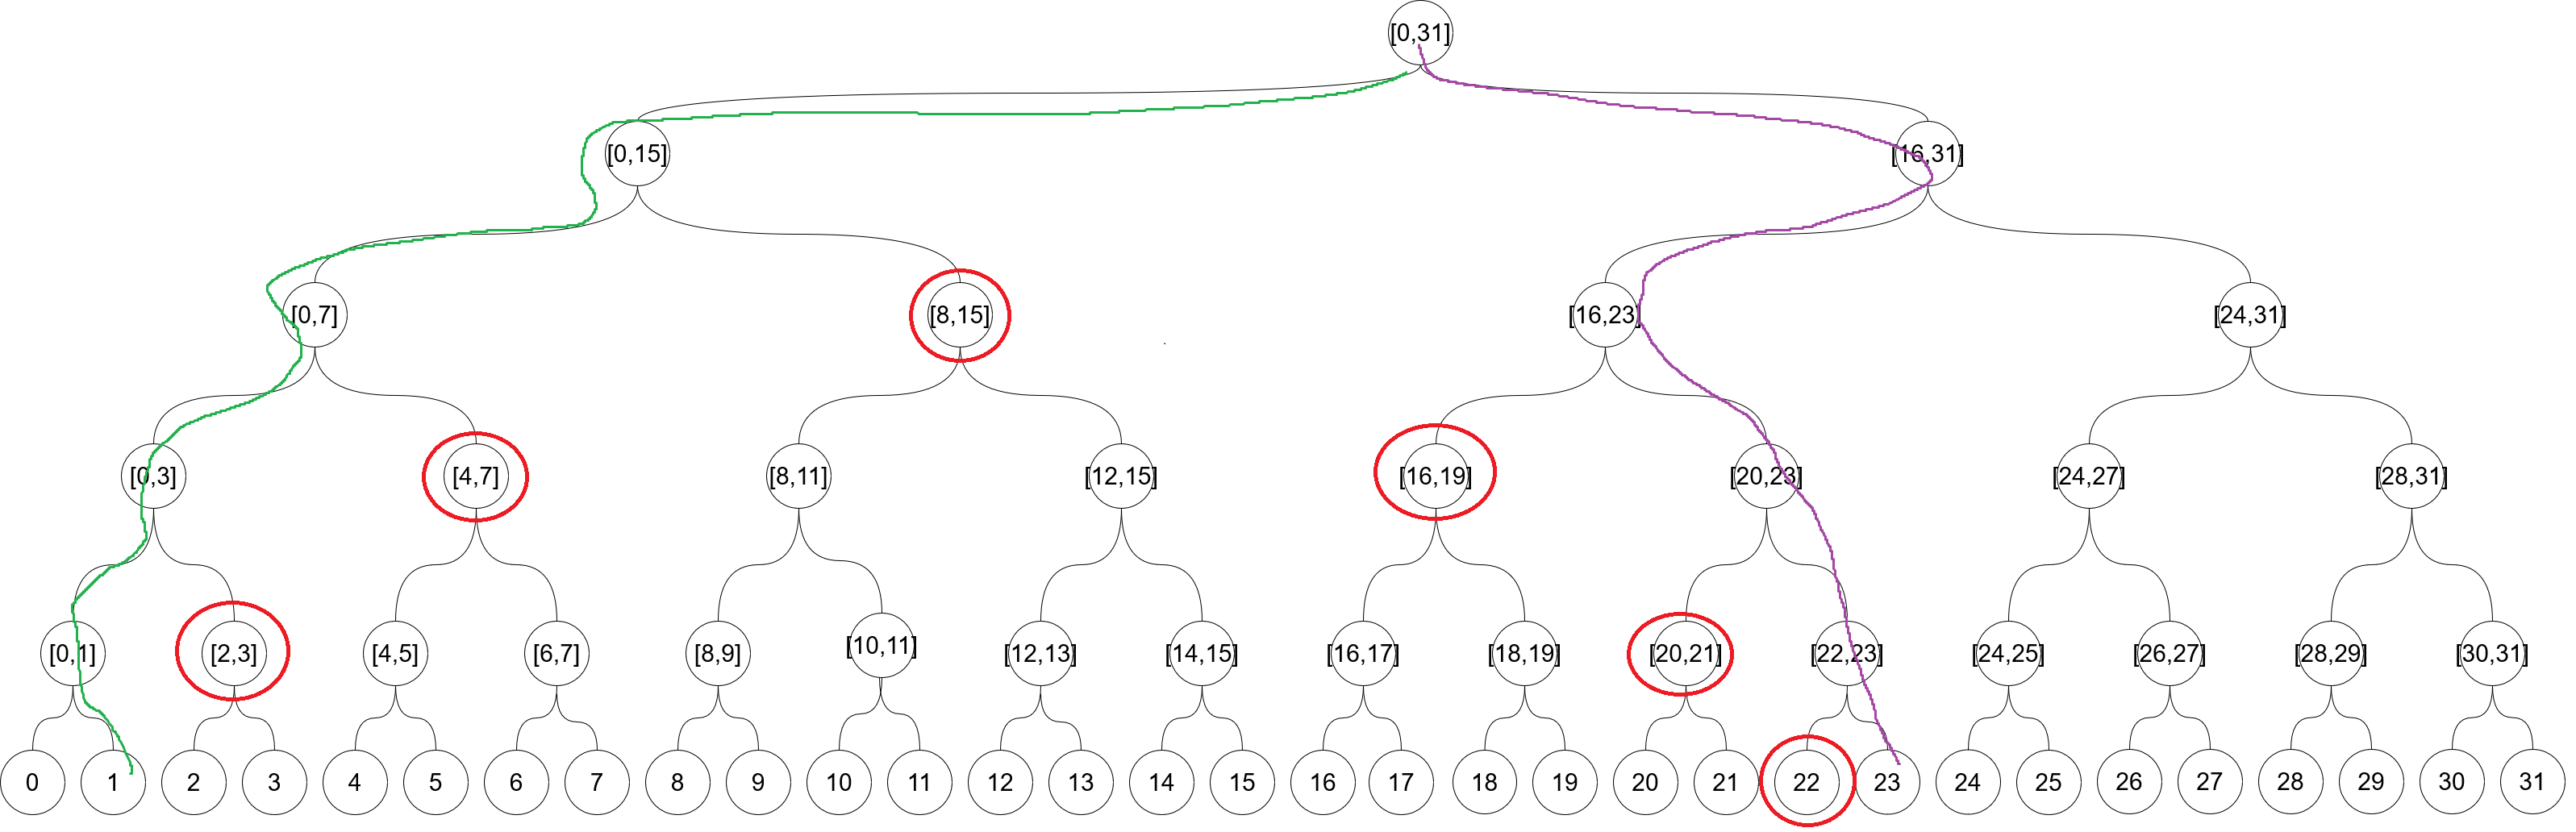
\includegraphics[width=.8\linewidth]{figures/disjoint_search_1.png}
    \caption{Range query search in hierarchical histograms}
    \label{fig:disjoint_se_1}
\end{figure}

\subsection{Continuous Observations}
The implementation for the continuous observations solution, takes four arguments $\epsilon$, the domain, the counts of each element in the domain and a degree. 
When running the implementation, the data structure makes a true continuous observations hierarchical histogram of the domain, and a tree with the same dimension, where it stores in the leaves the sum of all the Laplace variables, needed for the corresponding leaf in true histogram. The true histogram and the tree with Laplace variables are then added together. To answer a range query, we need the continuous count from the last element in the range and subtract it from continuous count from the first element of the range. To get the continuous count we use the method described in section \ref{decom}. 

\subsection{Local Hierarchical Histograms}
The implementation for the Local Hierarchical Histograms, takes 4 arguments $\epsilon$, the domain, the counts of each element in the domain and a degree. 
When running the implementation, the data structure makes an empty full ary tree with the given degree. It then goes for every count of every element in the domain. We sample a random level and use the frequency oracle on this level and, and adds this to the corresponding level of the full ary tree. To answer a range query, we need to get the nodes corresponding to the B-adic decomposition, as described in section \ref{decom}. We then sum up what the frequency estimator response with on the nodes and times this with the height of the tree.

\subsection{Testing}
The testing strategy was unit testing. Some of the things in the data structures can be quite difficult to use unit testing, as they rely on randomness. To test the random things I instead chose to do some sanity checks and self inspect to see if the randomness performed as 'expected'. A example of this was testing the 'randomness' to see if we got the correct result. We could run the same range query on 100 data structure with the same parameters. We could then get a CDF of the results and check if they match with the expectation. Also as a consequence of the composition theorem, if we average the 100 results we would get a DP algorithm with privacy guarantee of $100\cdot\epsilon$ that we used in our data structure. These sanity check for the data structure implementations can be seen in Figures \ref{fig:flat_sainty} and \ref{fig:hh_sainty}.
\begin{figure}
\begin{subfigure}{.5\textwidth}
  \centering
  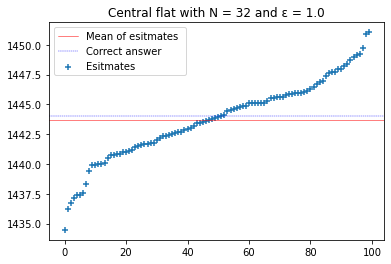
\includegraphics[width=\linewidth]{figures/tests/cen_flat/index.png}
  \caption{Sanity check central flat data structures}
  \label{fig:test_c_flat}
\end{subfigure}%
\begin{subfigure}{.5\textwidth}
  \centering
  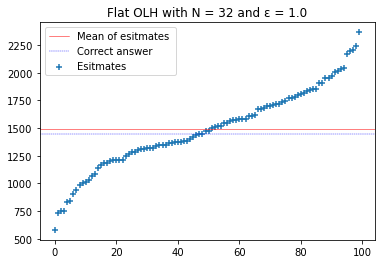
\includegraphics[width=\linewidth]{figures/tests/local_flat/index.png}
  \caption{Sanity check local flat data structures}
  \label{fig:test_l_flat}
\end{subfigure}%
\caption{Sanity checks of data structures}
\label{fig:flat_sainty}
\end{figure}

\begin{figure}
\begin{subfigure}{.5\textwidth}
  \centering
  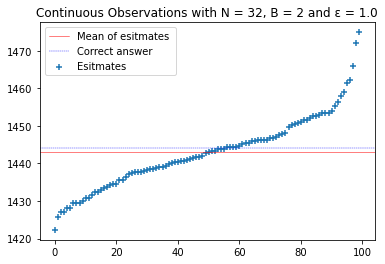
\includegraphics[width=\linewidth]{figures/tests/cen_hh/b=2.png}
  \caption{Sanity check continuous observations structures}
  \label{fig:test_c_flat}
\end{subfigure}%
\begin{subfigure}{.5\textwidth}
  \centering
  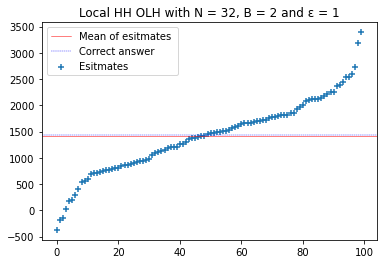
\includegraphics[width=\linewidth]{figures/tests/local_hh/b=2.png}
  \caption{Sanity check local HH data structures}
  \label{fig:test_l_flat}
\end{subfigure}%
\caption{Sanity checks of data structures}
\label{fig:hh_sainty}
\end{figure}


\section{Experiments and results}
\subsection{Dataset}
The dataset used for experiments describes the number of people visiting different public libraries in Aarhus. The data consist of three columns. The first column contains the dates with timestamps in the format 'Y-m-dTtimestamp', and the second column is the number of people who went into the library in the given hour. The third column is ID string which identifies what library in Aarhus the datapoint belongs to. There were 16 different libraries in the dataset. I chose to sum up the number of visitors on a day instead of having them as individual hours. In the experiments the data from library with id code of 775147.

In the data, some dates were missing due to holidays and etc. This was corrected by adding the missing dates and set the number of visitors for that day to $0$.  The data was loaded into a Postgres database. This allows for easier access to the data when doing experiments. 

The dataset comes from \url{https://www.opendata.dk/city-of-aarhus/besogstal-og-abningstider-for-aarhus-kommunes-biblioteker#resource-bes\%C3\%B8g} under section Besøg (2014-2019).

\subsection{Generation of range queries of specific a length}
For the experiments and test of the different data structures, we would need different range queries of the same length. These queries was generated at random, by sampling a date uniformly at random of the domain and adding the length of the range query to this date. We then check if the new date is still in the domain of the dates. If not we re-sample and do the same thing until a range has been sampled.  

\subsection{Flat solutions with varying length of queries}
As we have shown in both the sections \ref{teo_cen_flat} about the central flat solution, the error of flat solutions scales linearly with the length of the queries. We also expect the error to scale with $\epsilon$. We made data structures with varying domain sizes $N$ and different privacy variables $\epsilon$, and ran range queries of varying length on the models to test this. The error measurement was the root mean error. 
We had the parameters, $\epsilon's = [2, 1.4, 1.2, 1, 0.8, 0.6, 0.4, 0.2]$, $n's = [32, 128, 256, 512, 1024, 2048]$. The length $r$ for the queries varied depending on the domain size $N$. The testing was performed with seven different lengths of queries. The lengths can be seen on table \ref{tab:cen_flat_r}. A total of $2500$ queries being estimated by 25 different data structures, 100 queries each data structure.
\begin{table}[H]
\centering
\begin{tabular}{|l|l|l|l|l|l|l|l|}
\hline
Domain size    & $r_1$ & $r_2$ & $r_3$ & $r_4$ & $r_5$ & $r_6$ & $r_7$\\ \hline
32   & 2        & 4        & 8        & 12       & 16       & 20       & 24       \\ \hline
128  & 20       & 40       & 50       & 60       & 70       & 80       & 90       \\ \hline
512  & 40       & 60       & 80       & 100      & 140      & 200      & 220      \\ \hline
1024 & 200      & 300      & 400      & 500      & 600      & 800      & 900      \\ \hline
2048 & 600      & 800      & 1000     & 1250     & 1500     & 1700     & 1800     \\ \hline
\end{tabular}
\caption{length of queries depending on $N$}
  \label{tab:cen_flat_r}
\end{table}

\subsubsection{Central flat solution}
Here we present the results for the central flat solution. All the plots of the errors can be seen in here \ref{app:cen_r}. I have chosen to display three of plots with the domain size $N$ being $[32,512,2048]$. All the plots show the same tendencies, so there is no reason to look at them all. Plots of the results can be seen on Figure \ref{fig:plt_cen_r}. We can quite clearly observe that the error grows linearly with the length of the query, as we would expect. This is further examined in plots of Figure \ref{fig:plt_cen_r_lin}. Here the errors (dependent variable) and the length of the queries (interdependent variable) are fitted with linear regression. All linear fitted functions have an $R^2$ value in the high $.9$ with the lowest $r^2$ being $0.9715$.  We can also see that the smaller the $\epsilon$ values gives a higher error, which its also in line with what we would expect.
\begin{figure}[H]
\centering
\begin{subfigure}{.3\textwidth}
  \centering
  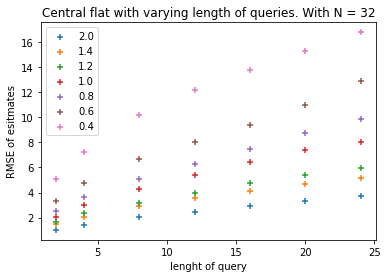
\includegraphics[width=\linewidth]{figures/central_flat/varying_r/cen_flat_varying_length_N=32.png}
  \caption{RMSE over $r$ for $N=32$}
  \label{fig:cen_r_sub1}
\end{subfigure}%
\begin{subfigure}{.3\textwidth}
  \centering
  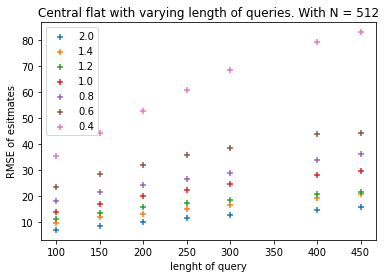
\includegraphics[width=\linewidth]{figures/central_flat/varying_r/cen_flat_varying_length_N=512.png}
  \caption{RMSE over of $r$ for $N=512$}
  \label{fig:cen_r_sub2}
\end{subfigure}
\begin{subfigure}{.3\textwidth}
  \centering
  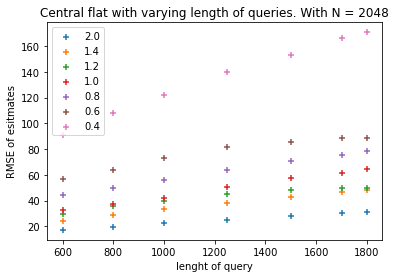
\includegraphics[width=\linewidth]{figures/central_flat/varying_r/cen_flat_varying_length_N=2048.png}
  \caption{RMSE over $r$ for $N=2028$}
  \label{fig:cen_r_sub3}
\end{subfigure}
\caption{Central flat plots with RMSE over $r$}
\label{fig:plt_cen_r}
\end{figure}

\begin{figure}[H]
\centering
\begin{subfigure}{.3\textwidth}
  \centering
  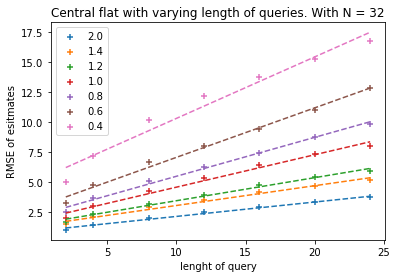
\includegraphics[width=\linewidth]{figures/central_flat/varying_r/cen_flat_varying_length_N_linear_=32.png}
  \caption{Linear fit of error for $N=32$}
  \label{fig:cen_r_sub1_lin}
\end{subfigure}%
\begin{subfigure}{.3\textwidth}
  \centering
  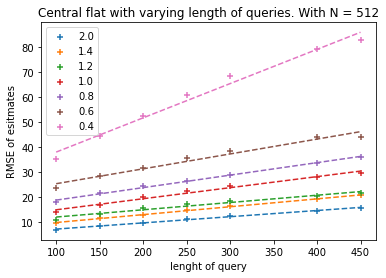
\includegraphics[width=\linewidth]{figures/central_flat/varying_r/cen_flat_varying_length_N_linear_=512.png}
  \caption{Linear fit of error for $N=512$}
  \label{fig:cen_r_sub2_lin}
\end{subfigure}
\begin{subfigure}{.3\textwidth}
  \centering
  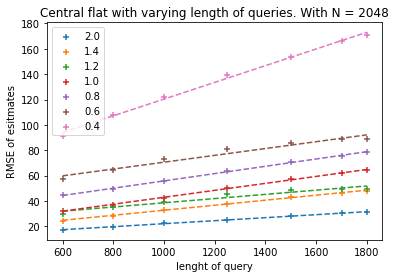
\includegraphics[width=\linewidth]{figures/central_flat/varying_r/cen_flat_varying_length_N_linear_=2048.png}
  \caption{Linear fit of error for $N=2028$}
  \label{fig:cen_r_sub3_lin}
\end{subfigure}
\caption{Central flat plots with RMSE as function of $r$}
\label{fig:plt_cen_r_lin}
\end{figure}

\subsubsection{Local Flat Solution}
Here we present the results for the local flat solution. All the plots of the errors can be seen in here \ref{app:loc_r}. I have chosen to display 3 of them with the domain size $N$ being $[32,512,2048]$. All the plots show the same tendencies, so there is no reason to look at them all. Plots of the results can be seen on Figure \ref{fig:plt_cen_r}. We can here observe that the error does not scale linearly with the length of the query, as we would expect, and as the theory states. It looks like it is scaling length of the query at the start but then stops, and the error decreases all of the sudden. It error seems more so to follow a second degree polynomial. This back up by the plots in Figures \ref{fig:plt_loc_r_lin_poly_2} and \ref{fig:plt_loc_r_lin_poly_1}. We can see the linear regression fits really poorly and the second degree polynomial fits much better. \\ \\ 
To understand why this is happening we have to look at the frequency oracle, so the frequency oracle either responds with the correct $z$ with a certain probability or it chooses a random $z\in\mathcal{Z}$, because of element $z$ of $\mathcal{Z}$ is counted once, where it belongs in the domain is just random. When we make a range query over a large percentage of the domain, it will not matter if responded truthfully about the location in the domain, as long as our u.a.r response was still in the part of the domain that is a part of the current range query, because it will then counted in this range either way. This is also evidently by when i did a range query over the whole domain with the flat solution. Every time it answered with the true answer (bearing in mind some floating point operations errors), because we count every element in the domain, but at wrong locations.\\ \\
This gives me some doubt about the differential privacy of this frequency oracle. If we assume a company did local DP survey where all their users responds with this implementation. We let the company do a range query on the whole domain, about how many of users satisfies property $y$. After one single day they get just a single new user, and run the same query. If the count of how many satisfies property $y$ goes up by one, we know with 100\% certainty that this new user satisfies property $y$.
\begin{figure}[H]
\centering
\begin{subfigure}{.4\textwidth}
  \centering
  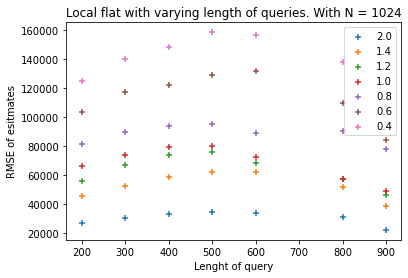
\includegraphics[width=\linewidth]{figures/local_flat/varying_r/loc_flat_varying_length_N=1024.png}
  \caption{RMSE over $r$ for $N=1024$}
  \label{fig:loc_r_sub1_1}
\end{subfigure}%
\begin{subfigure}{.4\textwidth}
  \centering
  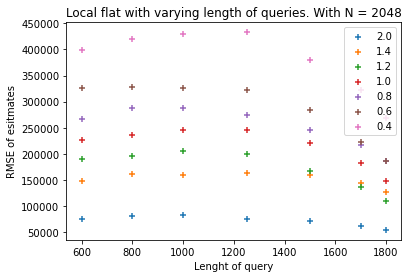
\includegraphics[width=\linewidth]{figures/local_flat/varying_r/loc_flat_varying_length_N=2048.png}
  \caption{RMSE over $r$ for $N=2028$}
  \label{fig:loc_r_sub3_2}
\end{subfigure}
\caption{Local flat plots with RMSE over $r$}
\label{fig:plt_loc_r}
\end{figure}


\begin{figure}[H]
\centering
\begin{subfigure}{.4\textwidth}
  \centering
  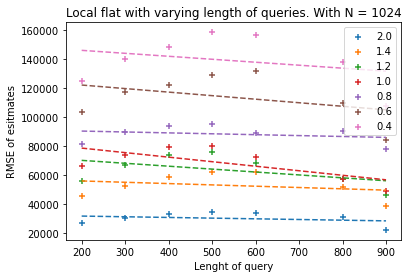
\includegraphics[width=\linewidth]{figures/local_flat/varying_r/loc_flat_varying_length_N_linear_=1024.png}
  \caption{Linear fit of error for $N=1024$}
  \label{fig:loc_r_sub1_lin_}
\end{subfigure}%
\begin{subfigure}{.4\textwidth}
  \centering
  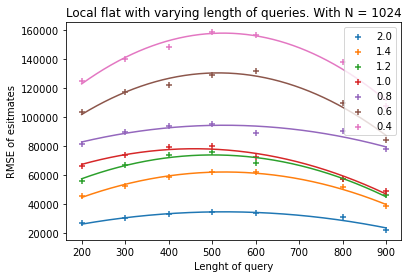
\includegraphics[width=\linewidth]{figures/local_flat/varying_r/loc_flat_varying_length_N_poly_=1024.png}
  \caption{Poly fit of error with  $N=1024$}
  \label{fig:loc_r_sub3_lin__}
\end{subfigure}
\caption{Linear regression fit of RMSE as function of $r$}
\label{fig:plt_loc_r_lin_poly_1}
\end{figure}

\begin{figure}[H]
\centering
\begin{subfigure}{.4\textwidth}
  \centering
  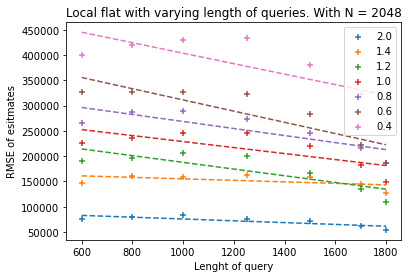
\includegraphics[width=\linewidth]{figures/local_flat/varying_r/loc_flat_varying_length_N_linear_=2048.png}
  \caption{Linear fit of error with $N=2048$}
  \label{fig:loc_r_sub2_lin}
\end{subfigure}%
\begin{subfigure}{.4\textwidth}
  \centering
  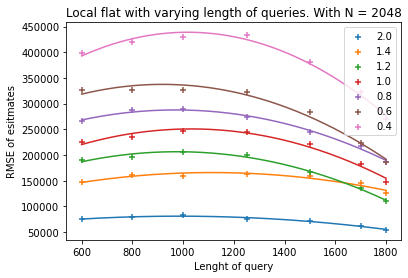
\includegraphics[width=\linewidth]{figures/local_flat/varying_r/loc_flat_varying_length_N_poly_=2048.png}
  \caption{Poly fit of error with $N=2048$ }
  \label{fig:loc_r_sub2_poly}
\end{subfigure}
\caption{Second degree polynomial fit of RMSE as function of $r$}
\label{fig:plt_loc_r_lin_poly_2}
\end{figure}


\subsection{Continuous observation impact of $\epsilon$ and degree}




\subsection{Local HH impact of $\epsilon$ and degree}




\newpage\subsection{Flat solutions vs HH solutions}
In these experiments, there were a total of $2500$ queries being estimated by 25 different data structures, 100 queries each data structure. As explain earlier the data structures for local hierarchical histogram resembles the data structures for continuous observation very closely. They both build on the same thought of imposing a heircay on intervals in the domain. I will therefore denote the continuous observation as hierarchical histogram, for the experiments in the next section.
\subsubsection{When does hierarchical histogram beat the flat solutions?}
The benefit of the hierarchical histogram approach over the baseline flat method comes from the fact that we, at some point, need to visit fewer nodes in HH than in the flat solutions. Sometimes we could answer a range range that is defined by a singe node in the HH where we would need many more a lot of point estimations in the flat solution. We have shown in a previous section that the number of nodes we need to visit in the HH depends on the height of the HH, which depends on the degree of the HH. The number of nodes we needed to visit in a HH is $(2B-1)h\alpha$ versus in the flat approach is the quantity r, when answering a range query. We have that $h=\log_B(|\mathcal{Z}|)+O(1)$ and $\alpha=\log_B(r)+O(1)$ from our previous section about local hierarchical histogram. Therefore we obtain an improvement over flat methods when $r>2\cdot B \log_B^2(|\mathcal{Z}|)$. \\ \\ I have plotted the maximum length of the queries that hierarchical histogram needs to beat flat solutions for various degrees of a hierarchical histogram. The plots of this can be seen in figure \ref{fig:benefit}. The HHs could potentially beat the flat solution earlier if the range matches the interval of one leaf in the tree. We can see from the plots that the HH might not beat the flat solutions for some combinations of $B$ and $|\mathcal{Z}|$ for example. When if pick $|\mathcal{Z}| = 64$ and $B=2$ the length for when the HH starts beating the flat solution is 144, which is impossible as it can maximum be 64. The length used for the experiments were HHs beats the flat can be seen in table \ref{flat_v_hh}. The length used for the experiments were flat beats the HHs can be seen in table \ref{hh_v_flat}. 
\begin{figure}[H]
     \centering
     \begin{subfigure}[b]{0.3\textwidth}
         \centering
         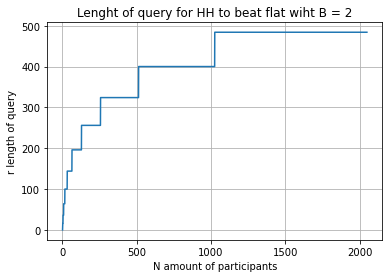
\includegraphics[width=\textwidth]{figures/benefit_2.png}
         \caption{Length needed for $B=2$}
         \label{fig:y equals x}
     \end{subfigure}
     \hfill
     \begin{subfigure}[b]{0.3\textwidth}
         \centering
         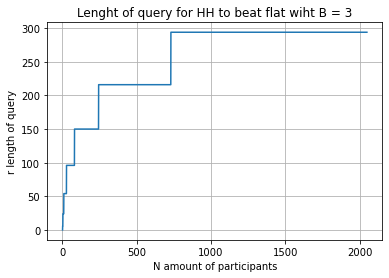
\includegraphics[width=\textwidth]{figures/benefit_3.png}
         \caption{Length needed for $B=3$}
         \label{fig:three sin x}
     \end{subfigure}
     \hfill
     \begin{subfigure}[b]{0.3\textwidth}
         \centering
         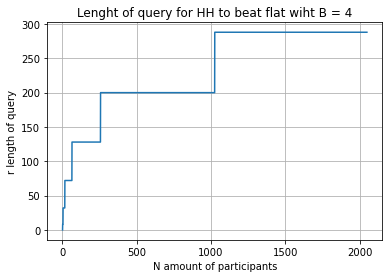
\includegraphics[width=\textwidth]{figures/benefit_4.png}
         \caption{Length needed for $B=4$}
         \label{fig:five over x}
     \end{subfigure}
        \caption{Length needed for HH to beat flat for various degrees}
        \label{fig:benefit}
\end{figure}
\begin{table}[H]
\centering
\begin{tabular}{|l|l|}
\hline
N    &  Length     \\ \hline
256  & Only possible to on whole range \\ \hline
512  & 324        \\ \hline
1024 & 400         \\ \hline
2048 & 484         \\ \hline
\end{tabular}
\quad
\begin{tabular}{|l|l|}
\hline
N    &  Length     \\ \hline
256  & 216 \\ \hline
512  & 216        \\ \hline
1024 & 294         \\ \hline
2048 & 294         \\ \hline
\end{tabular}
\quad
\begin{tabular}{|l|l|}
\hline
N    &  Length     \\ \hline
256  & 128 \\ \hline
512  & 200        \\ \hline
1024 & 200         \\ \hline
2048 & 288         \\ \hline
\end{tabular}
\caption{Length of queries for HH to beat flat with $B=2$, $B=3$ and $B=4$ respectively}
\label{flat_v_hh}
\end{table}
\begin{table}[H]
\centering
\begin{tabular}{|l|l|}
\hline
N    &  Length     \\ \hline
32  & 6 \\ \hline
128  & 9 \\ \hline
256  & 24 \\ \hline
512  & 35        \\ \hline
1024 & 44         \\ \hline
2048 & 64         \\ \hline
\end{tabular}
\caption{Length of queries for flat to beat HH with different domain sizes}
\label{hh_v_flat}
\end{table}

\subsubsection{Flat solutions beating the hierarchical histogram solutions}
Here we present the results for when the flat solutions should beat hierarchical histogram solutions, in both local and central differential privacy model. All the plots of the errors can be seen here \ref{app:cen_flat_over}. We have chosen to present six the plots, three for both the local and central solutions. As all the plots show the same tendencies, there is no reason to look at them all. In the plots i have chosen to look at we domain sizes $N\in[32,512,2048]$, this means the length of the queries would be $N\in[6,35,64]$ respectively for the domain sizes. In the plots, the RMSE value for the queries of a specific length is plotted over the eight different epsilon values. $\epsilon$ takes the values $\epsilon\in[2, 1.4, 1.2, 1, 0.8, 0.6, 0.4, 0.2]$.  The plots for the central models can be seen on figure \ref{fig:cen_flat_hh}. The plots for the local models can be seen on figure \ref{fig:loc_flat_hh}. \\ \\
We can see that the central models follow what we would expect, but the local models does not. In the central case we can clearly see that the flat solution beats hierarchical histogram solution. We can also see that the lowest RMSE value of the hierarchical histogram data structures is the one with the largest degree, this line with the theory.\\ \\
In the local case only for $N=32$, the local flat solution beats the local hierarchical histogram. For $N=512$ it is beaten hierarchical histogram solution with degree two and three. For $N=2048$ it is beaten by every hierarchical histogram solution. One potential reason for this, could be that the range queries represented a exactly one node in the hierarchical histogram, but if this was the case we would expect similar results would have been happened for the central models. This leads to think something else is the cause for this result. Another potential reason could be, that we know from the section \ref{freq}, the variance in of a element in the domain depends upon how many contributes to the mechanism. So the variance would be really high for each element in the flat solution as every one contributes to the mechanism if there are a lot in the domain. Where in the hierarchical histogram the variance would be spread uniformly out over the mechanism for each level. Therefore the variance of mechanism at each of the levels would be lower. This sort of backed of see the 
\begin{figure}[H]
\centering
\begin{subfigure}{.3\textwidth}
  \centering
  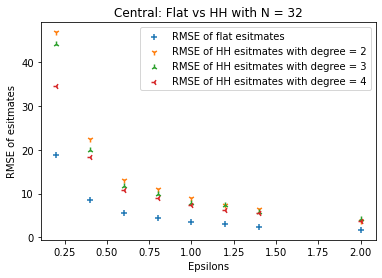
\includegraphics[width=\linewidth]{figures/central_flat_hh/flat_beat_hh_N=32.png}
  \caption{$N=32$}
  \label{fig:cen_flat_hh1}
\end{subfigure}%
\begin{subfigure}{.3\textwidth}
  \centering
  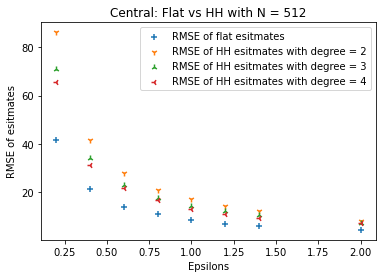
\includegraphics[width=\linewidth]{figures/central_flat_hh/flat_beat_hh_N=512.png}
  \caption{$N=512$}
  \label{fig:cen_flat_hh2}
\end{subfigure}%
\begin{subfigure}{.3\textwidth}
  \centering
  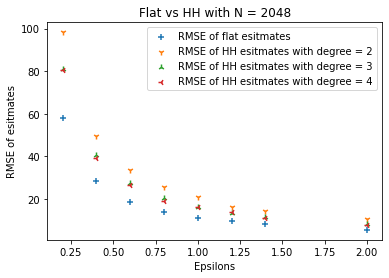
\includegraphics[width=\linewidth]{figures/central_flat_hh/flat_beat_hh_N=2048.png}
  \caption{$N=2048$}
  \label{fig:cen_flat_hh3}
\end{subfigure}
\caption{Central flat beating central HH}
\label{fig:cen_flat_hh}
\end{figure}
\begin{figure}[H]
\centering
\begin{subfigure}{.3\textwidth}
  \centering
  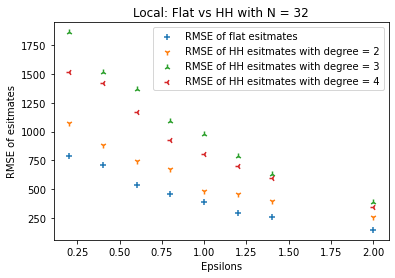
\includegraphics[width=\linewidth]{figures/local_flat_hh/flat_beat_hh_N=32.png}
  \caption{$N=32$}
  \label{fig:loc_flat_hh1}
\end{subfigure}%
\begin{subfigure}{.3\textwidth}
  \centering
  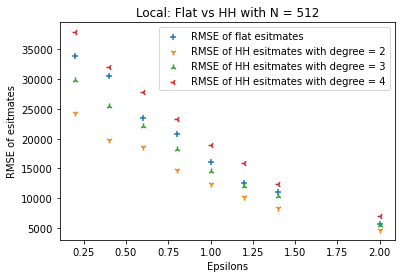
\includegraphics[width=\linewidth]{figures/local_flat_hh/flat_beat_hh_N=512.png}
  \caption{$N=512$}
  \label{fig:loc_flat_hh2}
\end{subfigure}%
\begin{subfigure}{.3\textwidth}
  \centering
  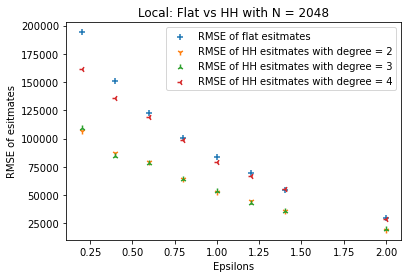
\includegraphics[width=\linewidth]{figures/local_flat_hh/flat_beat_hh_N=2048.png}
  \caption{$N=2048$}
  \label{fig:loc_flat_hh3}
\end{subfigure}
\caption{Loacl flat beating local HH}
\label{fig:loc_flat_hh}
\end{figure}


\subsubsection{Hierarchical histogram solutions beating flat solutions}
Here we present the results for when the flat solutions should beat hierarchical histogram solutions, in both local and central differential privacy model. We have chosen to present six the plots, three for both the local and central solutions. As all the plots show the same tendencies, there is no reason to look at them all. In the plots i have chosen to look at we domain sizes $N\in[256,512,2048]$ all with degree $B=4$, this means the length of the queries would be $N\in[128, 200, 288]$ respectively for the domain sizes. In the plots, the RMSE value for the queries of a specific length is plotted over the eight different epsilon values. $\epsilon$ takes the values $\epsilon\in[2, 1.4, 1.2, 1, 0.8, 0.6, 0.4, 0.2]$.  The plots for the central models can be seen on figure \ref{fig:cen_hh_flat}. The plots for the local models can be seen on figure \ref{fig:loc_hh_flat}. We can clearly see that the hierarchical histogram solutions  beats flat solutions as expected. The margin that is not that wide in the central case, where the margin but with the 
\begin{figure}[H]
\centering
\begin{subfigure}{.3\textwidth}
  \centering
  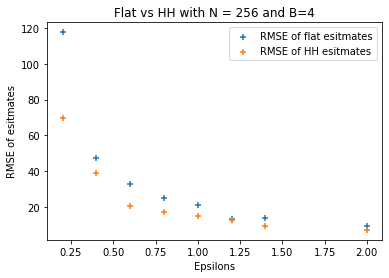
\includegraphics[width=\linewidth]{figures/central_hh_flat/hh_beat_flat=256_B=4.png}
  \caption{$N=256$ and $B=4$}
  \label{fig:cen256}
\end{subfigure}%
\begin{subfigure}{.3\textwidth}
  \centering
  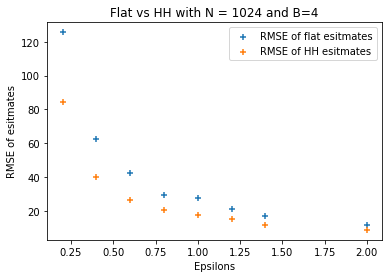
\includegraphics[width=\linewidth]{figures/central_hh_flat/hh_beat_flat=1024_B=4.png}
  \caption{$N=512$ and $B=4$}
  \label{fig:cen1024}
\end{subfigure}%
\begin{subfigure}{.3\textwidth}
  \centering
  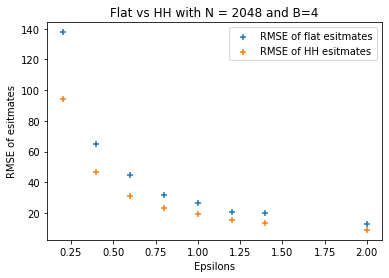
\includegraphics[width=\linewidth]{figures/central_hh_flat/hh_beat_flat=2048_B=4.png}
  \caption{$N=2048$ and $B=4$}
  \label{fig:cen2048}
\end{subfigure}
\caption{Central hierarchical histogram beating central flat solution}
\label{fig:cen_hh_flat}
\end{figure}
\begin{figure}[H]
\centering
\begin{subfigure}{.3\textwidth}
  \centering
  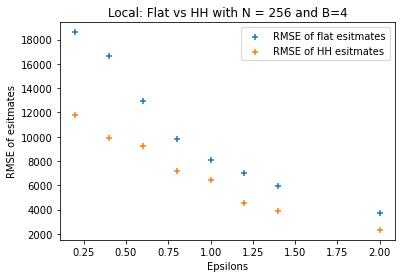
\includegraphics[width=\linewidth]{figures/local_hh_flat/hh_beat_flat=256_B=4.png}
  \caption{$N=256$ and $B=4$}
  \label{fig:loc256}
\end{subfigure}%
\begin{subfigure}{.3\textwidth}
  \centering
  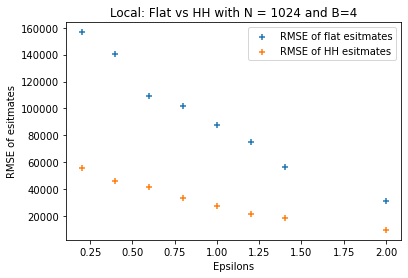
\includegraphics[width=\linewidth]{figures/local_hh_flat/hh_beat_flat=1024_B=4.png}
  \caption{$N=512$ and $B=4$}
  \label{fig:loc1024}
\end{subfigure}%
\begin{subfigure}{.3\textwidth}
  \centering
  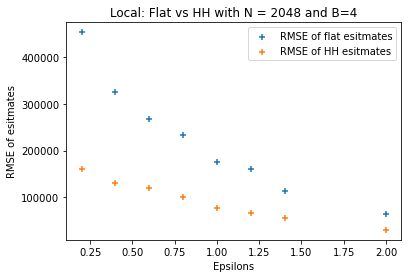
\includegraphics[width=\linewidth]{figures/local_hh_flat/hh_beat_flat=2048_B=4.png}
  \caption{$N=2048$ and $B=4$}
  \label{fig:loc2048}
\end{subfigure}
\caption{Local hierarchical histogram beating local flat solution}
\label{fig:loc_hh_flat}
\end{figure}

\newpage\subsection{Local vs Central}
In this section we want to see what happens in the error when we go from the central to the local model. The queries used to examine this is the same from the previous section. We $\epsilon\in[2, 1.4, 1.2, 1, 0.8, 0.6, 0.4, 0.2]$ in our data structures. We would expect that the error would be worse in the local solutions. This is also what we observe in the plots both for the flat solutions in Figure \ref{fig:chh_hh_flat} and the HH solution in Figure \ref{fig:hhhh_flat}. The extend of how much worse local solution is quite surprising. In the plots the errors for the central solution is pretty much a straight line at the bottom of the plot around 0 to 200, wheres the with the errors of the local solutions are are in the 10s of thousands. 
\begin{figure}[H]
\centering
\begin{subfigure}{.3\textwidth}
  \centering
  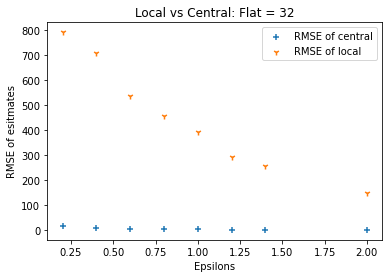
\includegraphics[width=\linewidth]{figures/cen_vs_loc/flat/flat_N=32.png}
  \caption{$N=32$}
  \label{fig:cen_vs32}
\end{subfigure}%
\begin{subfigure}{.3\textwidth}
  \centering
  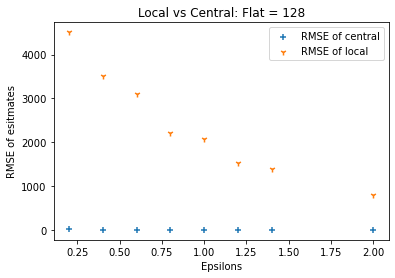
\includegraphics[width=\linewidth]{figures/cen_vs_loc/flat/flat_N=128.png}
  \caption{$N=128$}
  \label{fig:cen_vs256}
\end{subfigure}%
\begin{subfigure}{.3\textwidth}
  \centering
  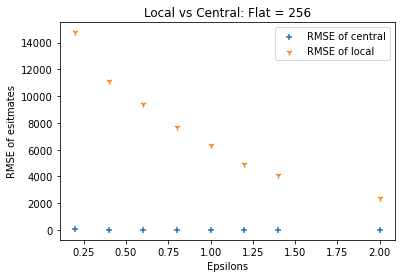
\includegraphics[width=\linewidth]{figures/cen_vs_loc/flat/flat_N=256.png}
  \caption{$N=256$}
  \label{fig:cen_vs1024}
\end{subfigure}
\caption{Central flat solution vs local flat solution}
\label{fig:chh_hh_flat}
\end{figure}
\begin{figure}[H]
\centering
\begin{subfigure}{.3\textwidth}
  \centering
  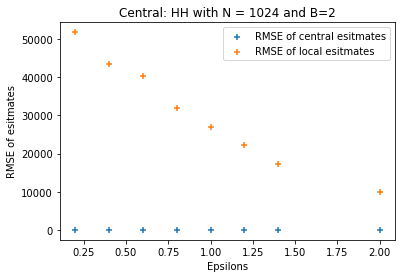
\includegraphics[width=\linewidth]{figures/cen_vs_loc/hh/hh_beat_flat=1024_B=2.png}
  \caption{$N=1024$ and $B=2$}
  \label{fig:hh_vs32}
\end{subfigure}%
\begin{subfigure}{.3\textwidth}
  \centering
  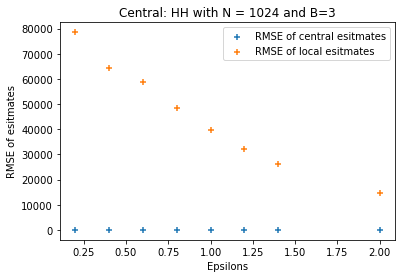
\includegraphics[width=\linewidth]{figures/cen_vs_loc/hh/hh_beat_flat=1024_B=3.png}
  \caption{$N=1024$ and $B=3$}
  \label{fig:hh_vs256}
\end{subfigure}%
\begin{subfigure}{.3\textwidth}
  \centering
  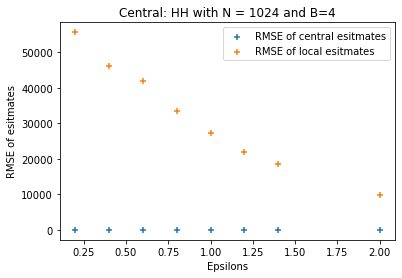
\includegraphics[width=\linewidth]{figures/cen_vs_loc/hh/hh_beat_flat=1024_B=4.png}
  \caption{$N=1024$ and $B=4$}
  \label{fig:hh_vs1024}
\end{subfigure}
\caption{Central HH solution vs local HH solution}
\label{fig:hhhh_flat}
\end{figure}



\section{Discussion}
As we can see from the experiments above
\section{Conclusion}
In this thesis, examined differential privacy, describe some of the concepts used in differential privacy, made a informal and formal definition of it. We proved proved the composition theorem about differential privacy. We have then describe four different data structures that support differential privacy for range counting. Two for both local and central differential privacy. \\
The two models in local and central differential privacy, build upon the same idea, one has 'flat' approach 
After implementing these four data structures we measured the error they estimation different range queries of varying length. They were then bench mark the local and central data structures against each other. We found that local had a higher error than the centrals ones, which was the theory describes.
% and central view of DP. We then implemented these data structures in python. We then benched marked 
% After proving the correctness, we implemented the algorithms in C++. We modified Dijkstra’s algorithm
% to be faster when searching for the shortest path to a single target, in the case where the target
% would not be the last vertex to visit.
% We analysed the Bellman Ford algorithm to have running time (E  V), while Dijkstra’s algorithm
% and A* search have running time O(E  lg(V)). Even though the running time would be asymptotically
% the same for Dijkstra’s algorithm and A* search we argued using heuristics that we in the
% non-worst-case would reach the vertex faster in A* search.
% We tested out the implementations and benchmarked them. We could then conclude that Bellman
% Ford grows extremely large in CPU-time by having the computational time of (V E). The Modified
% Dijkstra’s algorithm and A* search did really well, however the A* search did even better on all 4
% graphs of dierent size.
% Finally we can conclude that it makes a huge impact which shortest path algorithm you’d use for
% e.g. calculating the shortest path on a road-map. If some user would have to wait 19 seconds for a
% road-map application to find the shortest path using Bellman Ford, the user would probably go look
% for a dierent, faster application online.
We 
Har jeg svaret, hvorfor gik det galt
Svar på problem statement
\section{Future work}
Due to lack of time, some test and experiments was left out. I would have liked to have test the implemented data structures against some know attacks, reconstruction attack in particular, firstly to check if they actually were differential private, and then see what effect $\epsilon$, would have on the attack. We could also have shown how to break my bad implementation of continuous observation.


\newpage\section{Bibliography}
\printbibliography[]
\newpage\section{Appendix}
\subsection{Implementation}\label{app:imp}
\subsubsection{Central flat solution}
\inputminted[fontsize=\footnotesize,linenos]{python}{py_files/cen_flat.py}
\subsubsection{Local flat solution}
\inputminted[fontsize=\footnotesize,linenos]{python}{py_files/flat_olh.py}
\subsubsection{Continuous Observation}
\inputminted[fontsize=\footnotesize,linenos]{python}{py_files/con_obs.py}
\subsubsection{Local Hierarchical Histograms}
\inputminted[fontsize=\footnotesize,linenos]{python}{py_files/local_hh_object.py}

\subsection{Benchmark results}

\subsubsection{Central flat plots with varying r}\label{app:cen_r}
\begin{table}[H]
\begin{tabular}{|l|l|l|l|l|l|l|l|l|}
\hline
Length & 2                   & 4 & 8 & 12 & 16 & 20 & 24 \\ \hline
r      & 0.995&0.993&0.994&0.992&0.996 & 0.996 & 0.983 \\ \hline
\end{tabular}
\end{table}

\begin{figure}[H]
\centering
\begin{subfigure}{.4\textwidth}
  \centering
  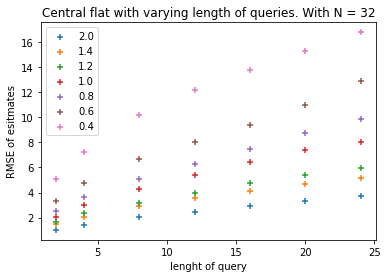
\includegraphics[width=\linewidth]{figures/central_flat/varying_r/cen_flat_varying_length_N=32.png}
  \caption{RMSE as function of $r$ for $N=32$}
  \label{fig:1}
\end{subfigure}%
\begin{subfigure}{.4\textwidth}
  \centering
  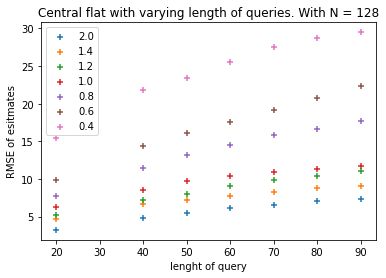
\includegraphics[width=\linewidth]{figures/central_flat/varying_r/cen_flat_varying_length_N=128.png}
  \caption{RMSE as function of $r$ for $N=128$}
  \label{fig:2}
\end{subfigure}
\begin{subfigure}{.4\textwidth}
  \centering
  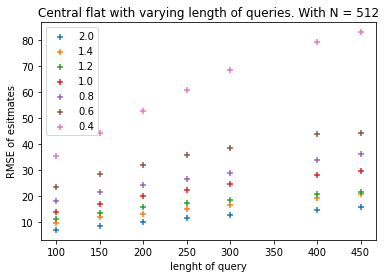
\includegraphics[width=\linewidth]{figures/central_flat/varying_r/cen_flat_varying_length_N=512.png}
  \caption{RMSE as function of $r$ for $N=512$}
  \label{fig:3}
  \begin{subfigure}{\textwidth}
  \centering
  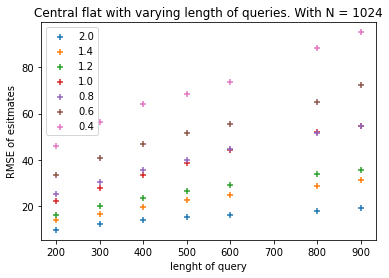
\includegraphics[width=\linewidth]{figures/central_flat/varying_r/cen_flat_varying_length_N=1024.png}
  \caption{RMSE as function of $r$ for $N=1024$}
  \label{fig:4}
\end{subfigure}
\begin{subfigure}{\textwidth}
  \centering
  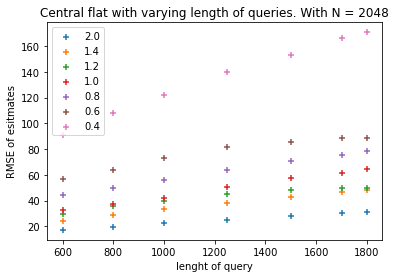
\includegraphics[width=\linewidth]{figures/central_flat/varying_r/cen_flat_varying_length_N=2048.png}
  \caption{RMSE as function of $r$ for $N=2028$}
  \label{fig:5}
\end{subfigure}
\caption{RMSE as function of $r$ and $N$}
\label{fig:6}
\end{subfigure}
\caption{RMSE as function of $r$ and $N$}
\label{fig:7}
\end{figure}
\begin{figure}[H]
\centering
\begin{subfigure}{.4\textwidth}
  \centering
  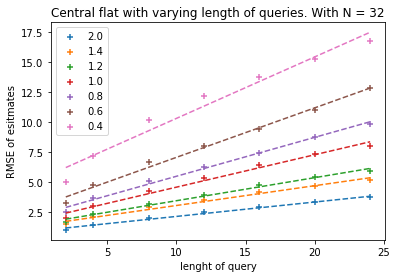
\includegraphics[width=\linewidth]{figures/central_flat/varying_r/cen_flat_varying_length_N_linear_=32.png}
  \caption{RMSE as function of $r$ for $N=32$}
  \label{fig:8}
\end{subfigure}%
\begin{subfigure}{.4\textwidth}
  \centering
  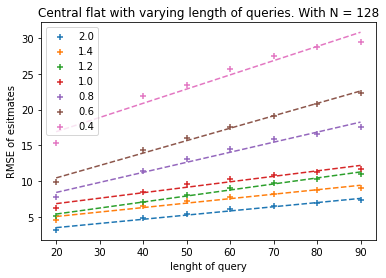
\includegraphics[width=\linewidth]{figures/central_flat/varying_r/cen_flat_varying_length_N_linear_=128.png}
  \caption{RMSE as function of $r$ for $N=128$}
  \label{fig:9}
\end{subfigure}
\begin{subfigure}{.4\textwidth}
  \centering
  \includegraphics[width=\linewidth]{figures/central_flat/varying_r/cen_flat_varying_length_N_linear_=512.png}
  \caption{RMSE as function of $r$ for $N=512$}
  \label{fig:10}
  \begin{subfigure}{\textwidth}
  \centering
  \includegraphics[width=\linewidth]{figures/central_flat/varying_r/cen_flat_varying_length_N_linear_=1024.png}
  \caption{RMSE as function of $r$ for $N=1024$}
  \label{fig:11}
\end{subfigure}
\begin{subfigure}{\textwidth}
  \centering
  \includegraphics[width=\linewidth]{figures/central_flat/varying_r/cen_flat_varying_length_N_linear_=2048.png}
  \caption{RMSE as function of $r$ for $N=2028$}
  \label{fig:12}
\end{subfigure}
\caption{RMSE as function of $r$ and $N$}
\label{fig:13}
\end{subfigure}
\caption{RMSE as function of $r$ and $N$}
\label{fig:14}
\end{figure}

\subsubsection{Local flat plots}\label{app:loc_r}
\begin{figure}[H]
\centering
\begin{subfigure}{.4\textwidth}
  \centering
  \includegraphics[width=\linewidth]{figures/local_flat/varying_r/loc_flat_varying_length_N=32.png}
  \caption{RMSE as function of $r$ for $N=32$}
  \label{fig:15}
\end{subfigure}%
\begin{subfigure}{.4\textwidth}
  \centering
  \includegraphics[width=\linewidth]{figures/local_flat/varying_r/loc_flat_varying_length_N=128.png}
  \caption{RMSE as function of $r$ for $N=128$}
  \label{fig:16}
\end{subfigure}
\begin{subfigure}{.4\textwidth}
  \centering
  \includegraphics[width=\linewidth]{figures/local_flat/varying_r/loc_flat_varying_length_N=512.png}
  \caption{RMSE as function of $r$ for $N=512$}
  \label{fig:17}
  \begin{subfigure}{\textwidth}
  \centering
  \includegraphics[width=\linewidth]{figures/local_flat/varying_r/loc_flat_varying_length_N=1024.png}
  \caption{RMSE as function of $r$ for $N=1024$}
  \label{fig:18}
\end{subfigure}
\begin{subfigure}{\textwidth}
  \centering
  \includegraphics[width=\linewidth]{figures/local_flat/varying_r/loc_flat_varying_length_N=2048.png}
  \caption{RMSE as function of $r$ for $N=2028$}
  \label{fig:19}
\end{subfigure}
\caption{RMSE as function of $r$ and $N$}
\label{fig:20}
\end{subfigure}
\caption{RMSE as function of $r$ and $N$}
\label{fig:21}
\end{figure}
\begin{figure}[H]
\centering
\begin{subfigure}{.4\textwidth}
  \centering
  \includegraphics[width=\linewidth]{figures/local_flat/varying_r/loc_flat_varying_length_N_linear_=32.png}
  \caption{RMSE as function of $r$ for $N=32$}
  \label{fig:22}
\end{subfigure}%
\begin{subfigure}{.4\textwidth}
  \centering
  \includegraphics[width=\linewidth]{figures/local_flat/varying_r/loc_flat_varying_length_N_linear_=128.png}
  \caption{RMSE as function of $r$ for $N=128$}
  \label{fig:23}
\end{subfigure}
\begin{subfigure}{.4\textwidth}
  \centering
  \includegraphics[width=\linewidth]{figures/local_flat/varying_r/loc_flat_varying_length_N_linear_=512.png}
  \caption{RMSE as function of $r$ for $N=512$}
  \label{fig:24}
  \begin{subfigure}{\textwidth}
  \centering
  \includegraphics[width=\linewidth]{figures/local_flat/varying_r/loc_flat_varying_length_N_linear_=1024.png}
  \caption{RMSE as function of $r$ for $N=1024$}
  \label{fig:25}
\end{subfigure}
\begin{subfigure}{\textwidth}
  \centering
  \includegraphics[width=\linewidth]{figures/local_flat/varying_r/loc_flat_varying_length_N_linear_=2048.png}
  \caption{RMSE as function of $r$ for $N=2028$}
  \label{fig:26}
\end{subfigure}
\caption{RMSE as function of $r$ and $N$}
\label{fig:27}
\end{subfigure}
\caption{RMSE as function of $r$ and $N$}
\label{fig:28}
\end{figure}
\begin{figure}[H]
\centering
\begin{subfigure}{.4\textwidth}
  \centering
  \includegraphics[width=\linewidth]{figures/local_flat/varying_r/loc_flat_varying_length_N_poly_=32.png}
  \caption{RMSE as function of $r$ for $N=32$}
  \label{fig:29}
\end{subfigure}%
\begin{subfigure}{.4\textwidth}
  \centering
  \includegraphics[width=\linewidth]{figures/local_flat/varying_r/loc_flat_varying_length_N_poly_=128.png}
  \caption{RMSE as function of $r$ for $N=128$}
  \label{fig:30}
\end{subfigure}
\begin{subfigure}{.4\textwidth}
  \centering
  \includegraphics[width=\linewidth]{figures/local_flat/varying_r/loc_flat_varying_length_N_poly_=512.png}
  \caption{RMSE as function of $r$ for $N=512$}
  \label{fig:31}
  \begin{subfigure}{\textwidth}
  \centering
  \includegraphics[width=\linewidth]{figures/local_flat/varying_r/loc_flat_varying_length_N_poly_=1024.png}
  \caption{RMSE as function of $r$ for $N=1024$}
  \label{fig:32}
\end{subfigure}
\begin{subfigure}{\textwidth}
  \centering
  \includegraphics[width=\linewidth]{figures/local_flat/varying_r/loc_flat_varying_length_N_poly_=2048.png}
  \caption{RMSE as function of $r$ for $N=2028$}
  \label{fig:33}
\end{subfigure}
\caption{RMSE as function of $r$ and $N$}
\label{fig:b}
\end{subfigure}
\caption{RMSE as function of $r$ and $N$}
\label{fig:34}
\end{figure}

\subsubsection{Central flat beating continuous observation}\label{app:cen_flat_over}
\begin{figure}[H]
\centering
\begin{subfigure}{.4\textwidth}
  \centering
  \includegraphics[width=\linewidth]{figures/central_flat_hh/flat_beat_hh_N=32.png}
  \caption{Linear fit of error for $N=32$}
  \label{fig:35}
\end{subfigure}%
\begin{subfigure}{.4\textwidth}
  \centering
  \includegraphics[width=\linewidth]{figures/central_flat_hh/flat_beat_hh_N=128.png}
  \caption{Linear fit of error for $N=128$}
  \label{fig:36}
\end{subfigure}
\begin{subfigure}{.4\textwidth}
  \centering
  \includegraphics[width=\linewidth]{figures/central_flat_hh/flat_beat_hh_N=256.png}
  \caption{Linear fit of error for $N=256$}
  \label{fig:37}
\end{subfigure}
\begin{subfigure}{.4\textwidth}
  \centering
  \includegraphics[width=\linewidth]{figures/central_flat_hh/flat_beat_hh_N=512.png}
  \caption{Linear fit of error for $N=512$}
  \label{fig:38}
\end{subfigure}%
\begin{subfigure}{.4\textwidth}
  \centering
  \includegraphics[width=\linewidth]{figures/central_flat_hh/flat_beat_hh_N=1024.png}
  \caption{Linear fit of error for $N=1024$}
  \label{fig:39}
\end{subfigure}
\begin{subfigure}{.4\textwidth}
  \centering
  \includegraphics[width=\linewidth]{figures/central_flat_hh/flat_beat_hh_N=2048.png}
  \caption{Linear fit of error for $N=2048$}
  \label{fig:40}
\end{subfigure}
\caption{Central flat beating continuous observation}
\label{99}
\end{figure}



\end{document}